% Bending operations

The test part undergoes a sequence of six bendings, with different angles and setups. Specifically, bending operations 1, 5, and 6 are performed at bending station 1 and undergoes a bending of 90° angle, whereas bending operations 2 and 3 are performed at bending station 2 with a bending of 135°, and the fourth bending operation is simply done to flatten the sheet metal part.

The first step before the bending for all bending operations is the correct alignment of the part in the backgauges of the bending machine. The bending machine program is automatically set by the terminal operating robot. Once the correct sequence is selected in the terminal of the bending machine, PLC send a signal to the KR1410 robot which gives permission to align the sheet in the backgauges.
Then only the KR1410 arm secures the part in the backgauges of the bending machine.

\begin{figure}[h]
    \centering
    \begin{subfigure}[b]{0.32\textwidth}
        \centering
        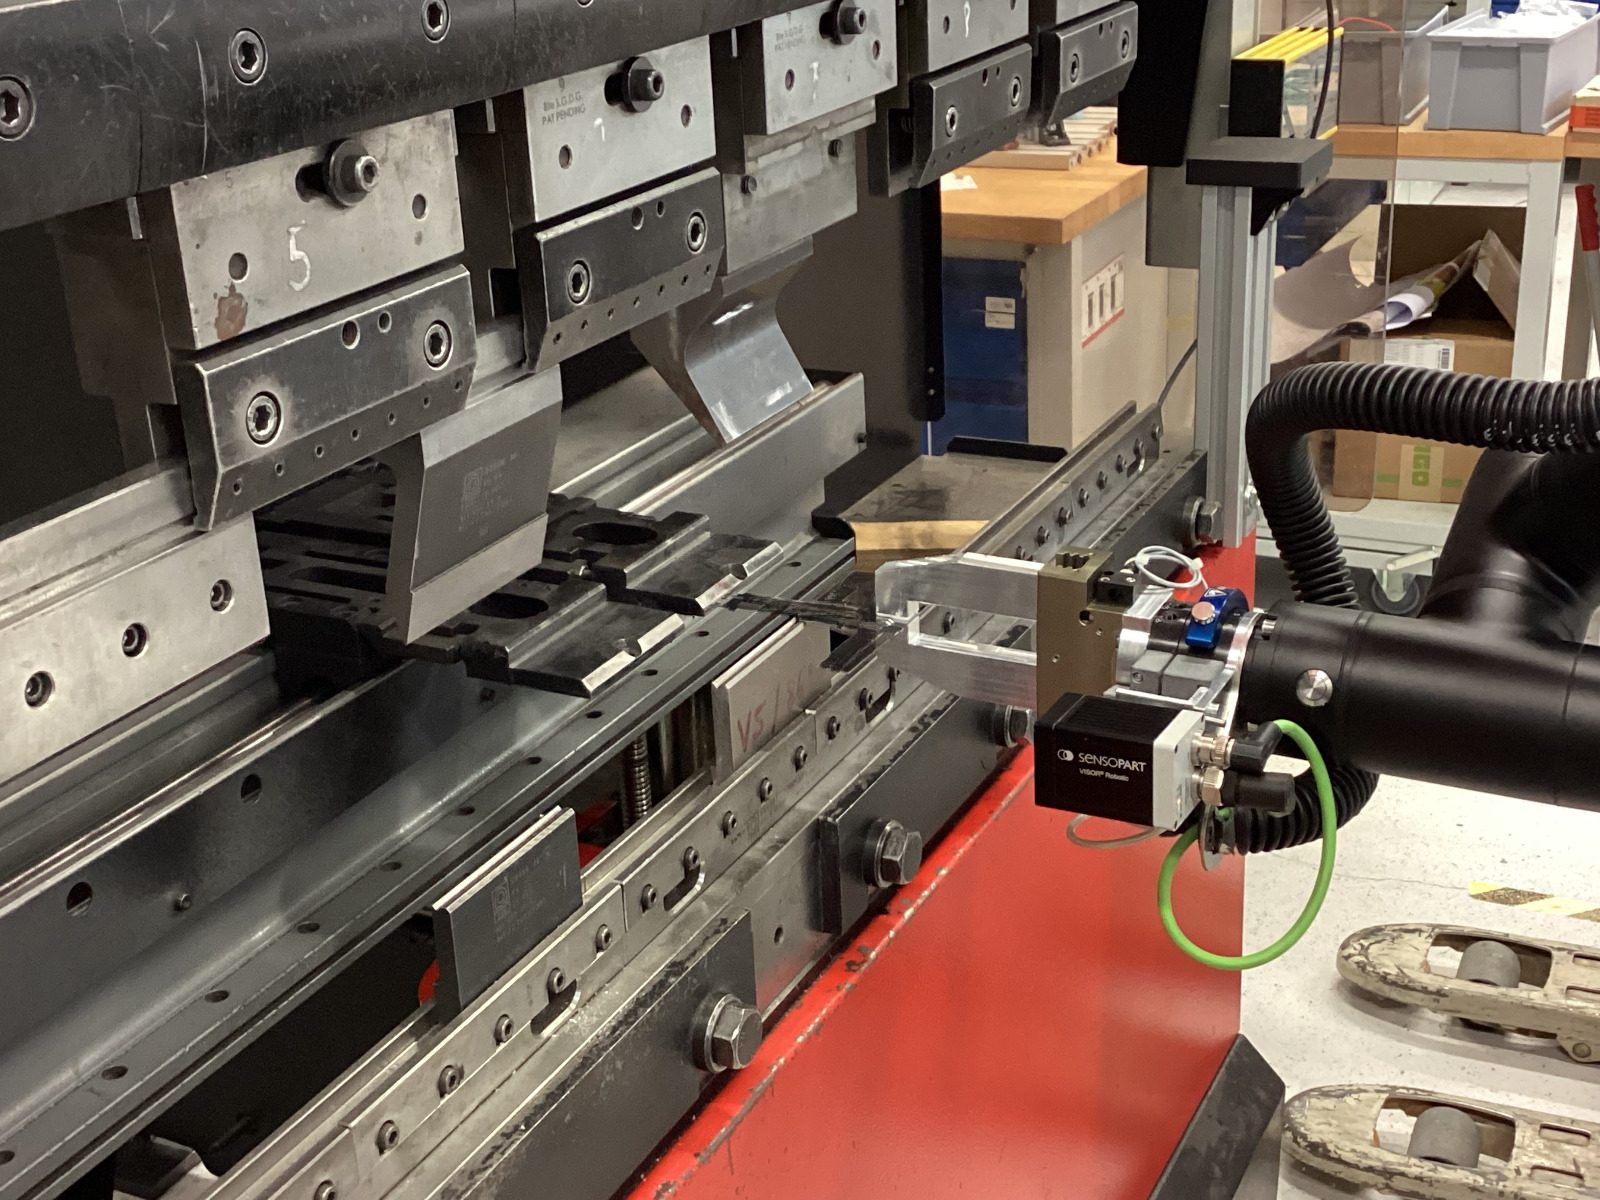
\includegraphics[width=\textwidth]{figures/bending/bending1-002.png}
        \caption{Go to bending station 1}
        \label{subfig:bending1-before}
    \end{subfigure}\hspace{0.1cm}
    \begin{subfigure}[b]{0.32\textwidth}
        \centering
        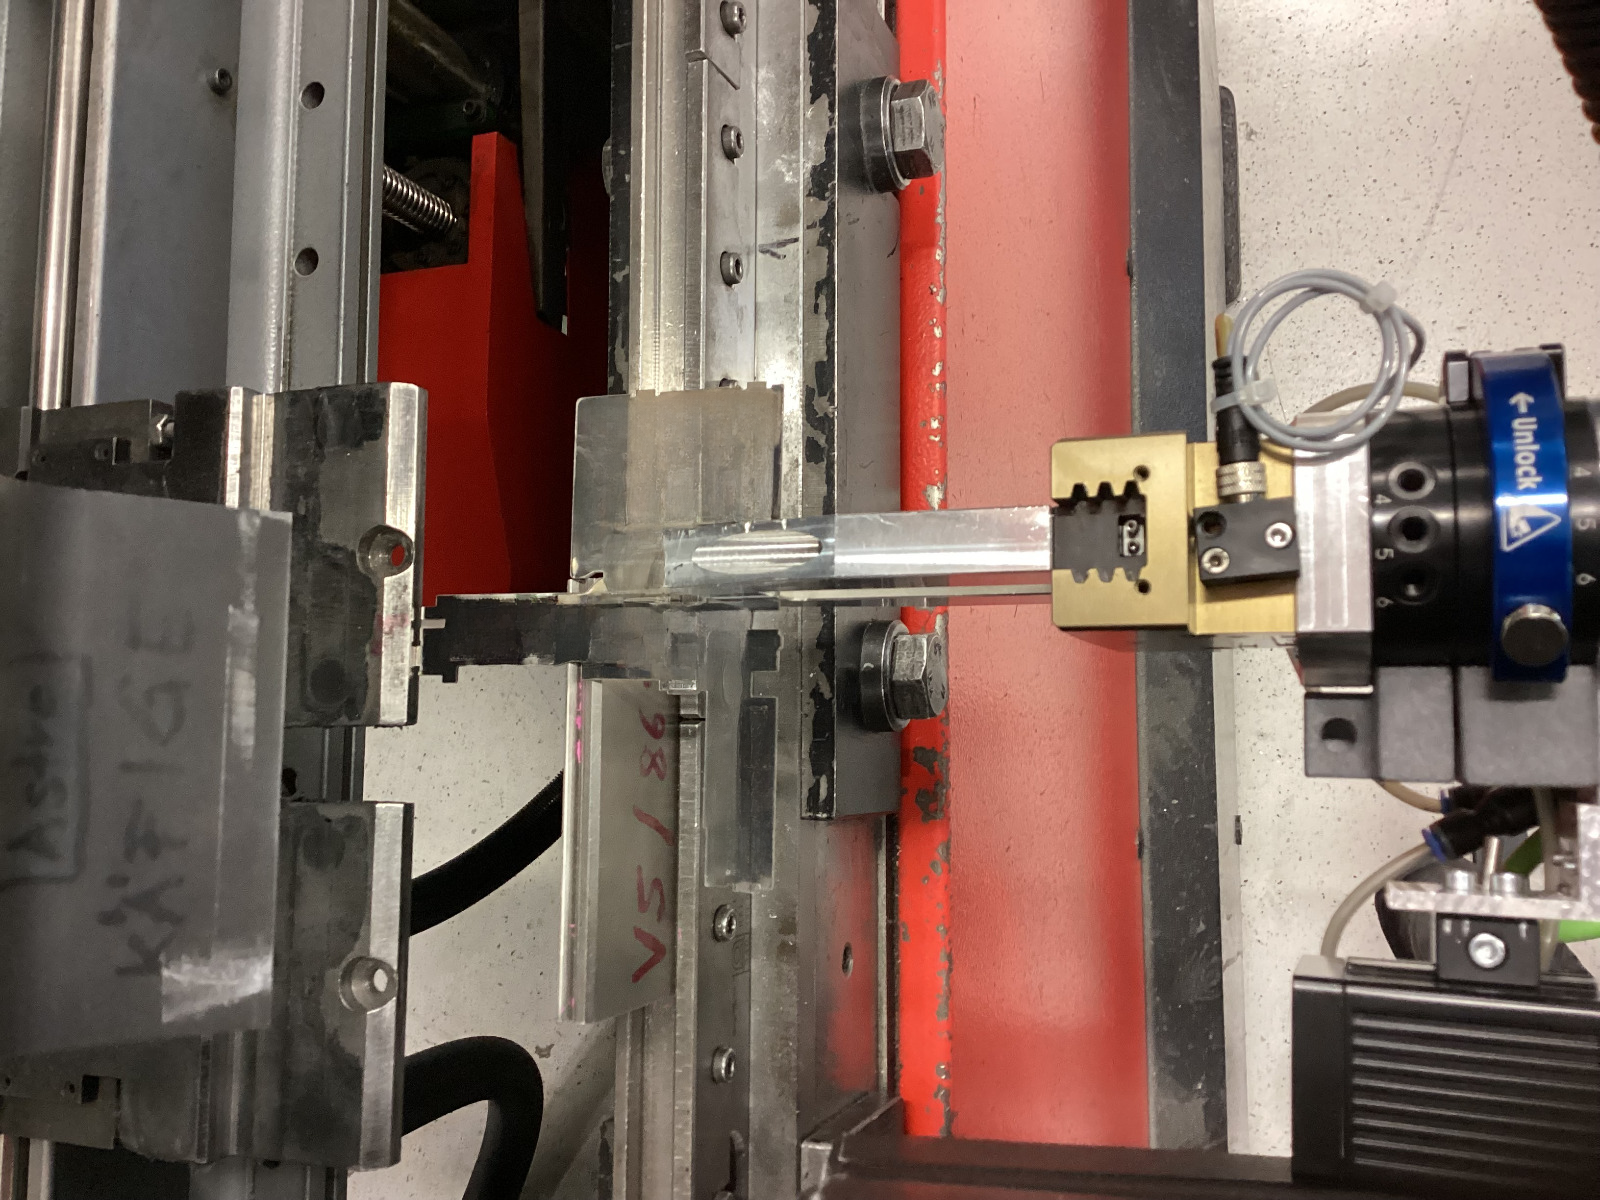
\includegraphics[width=\textwidth]{figures/bending/bending1-003.png}
        \caption{bend the sheet metal part}
        \label{subfig:bending1}
    \end{subfigure}\hspace{0.1cm}
    \begin{subfigure}[b]{0.32\textwidth}
        \centering
        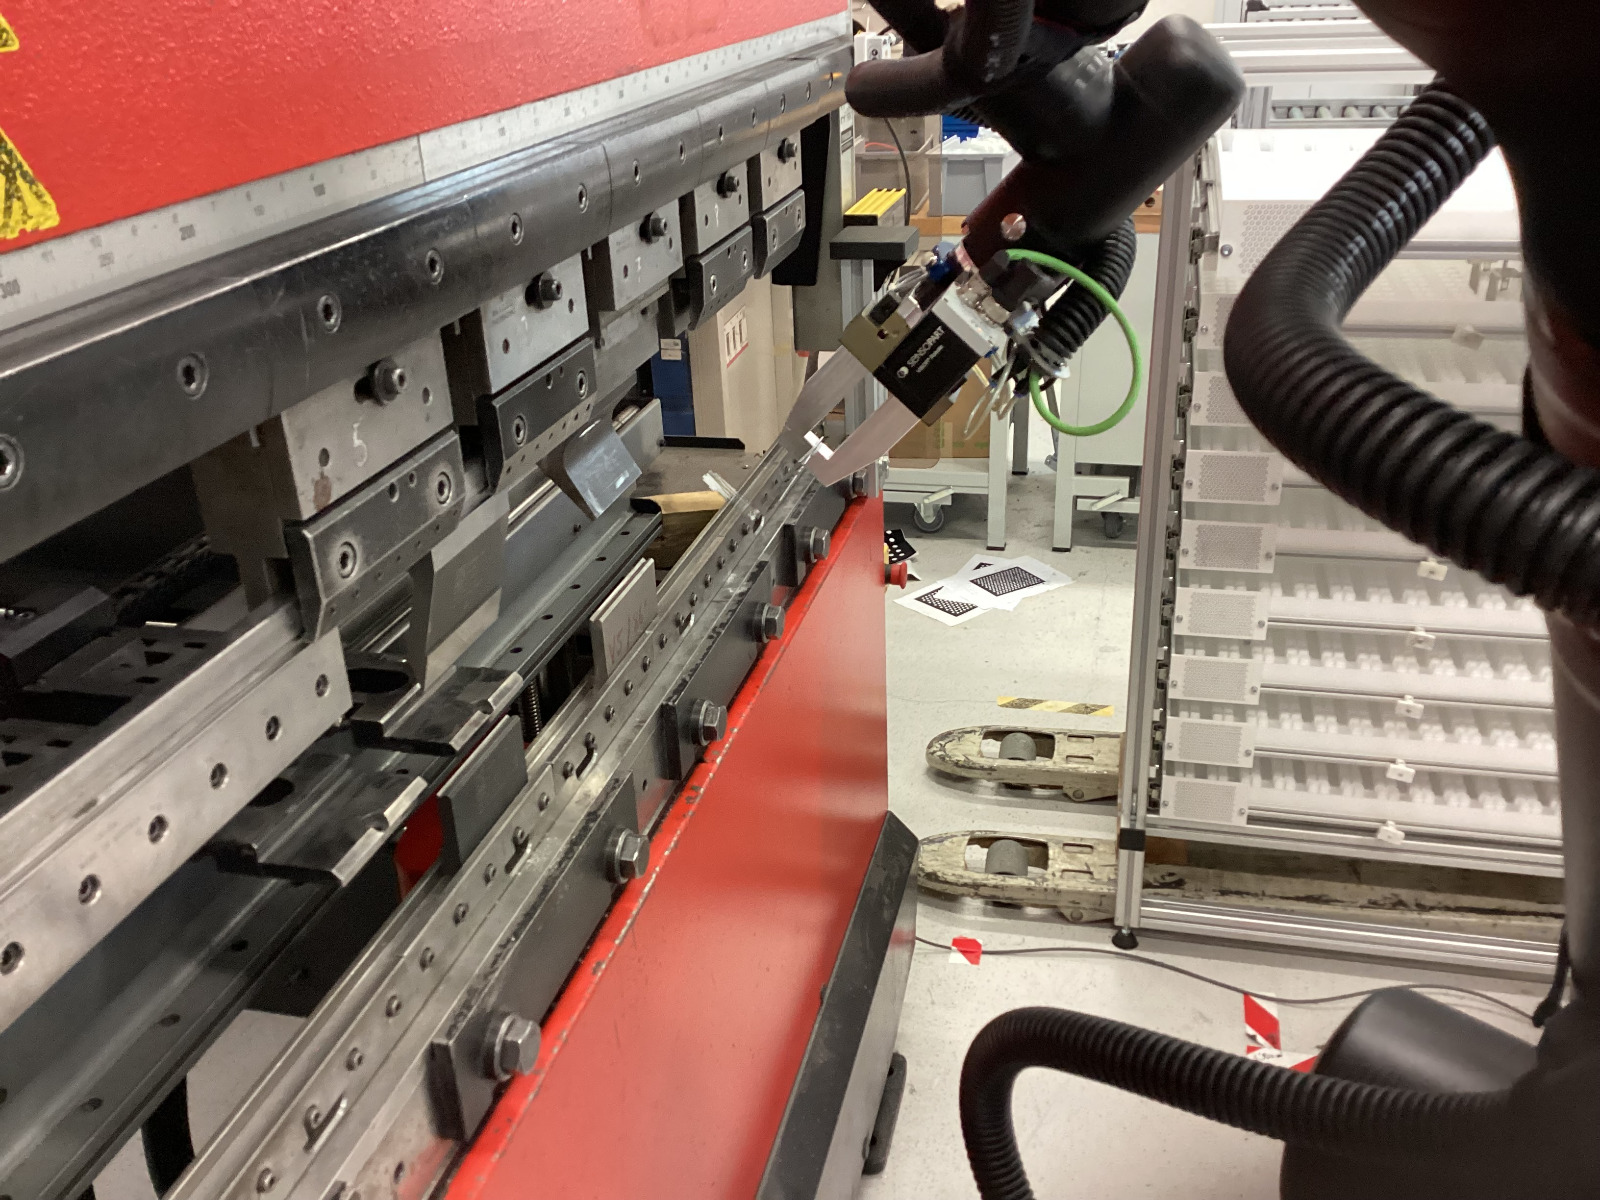
\includegraphics[width=\textwidth]{figures/bending/bending1-001.png}
        \caption{take away the bent sheet}
        \label{subfig:bending1-after}
    \end{subfigure}\hspace{0.1cm}
    \caption{Bending operation number 1 at bending station 1}
    \label{fig:bending-operation-1}
\end{figure}

\begin{figure}[h]
    \centering
    \begin{subfigure}[b]{0.32\textwidth}
        \centering
        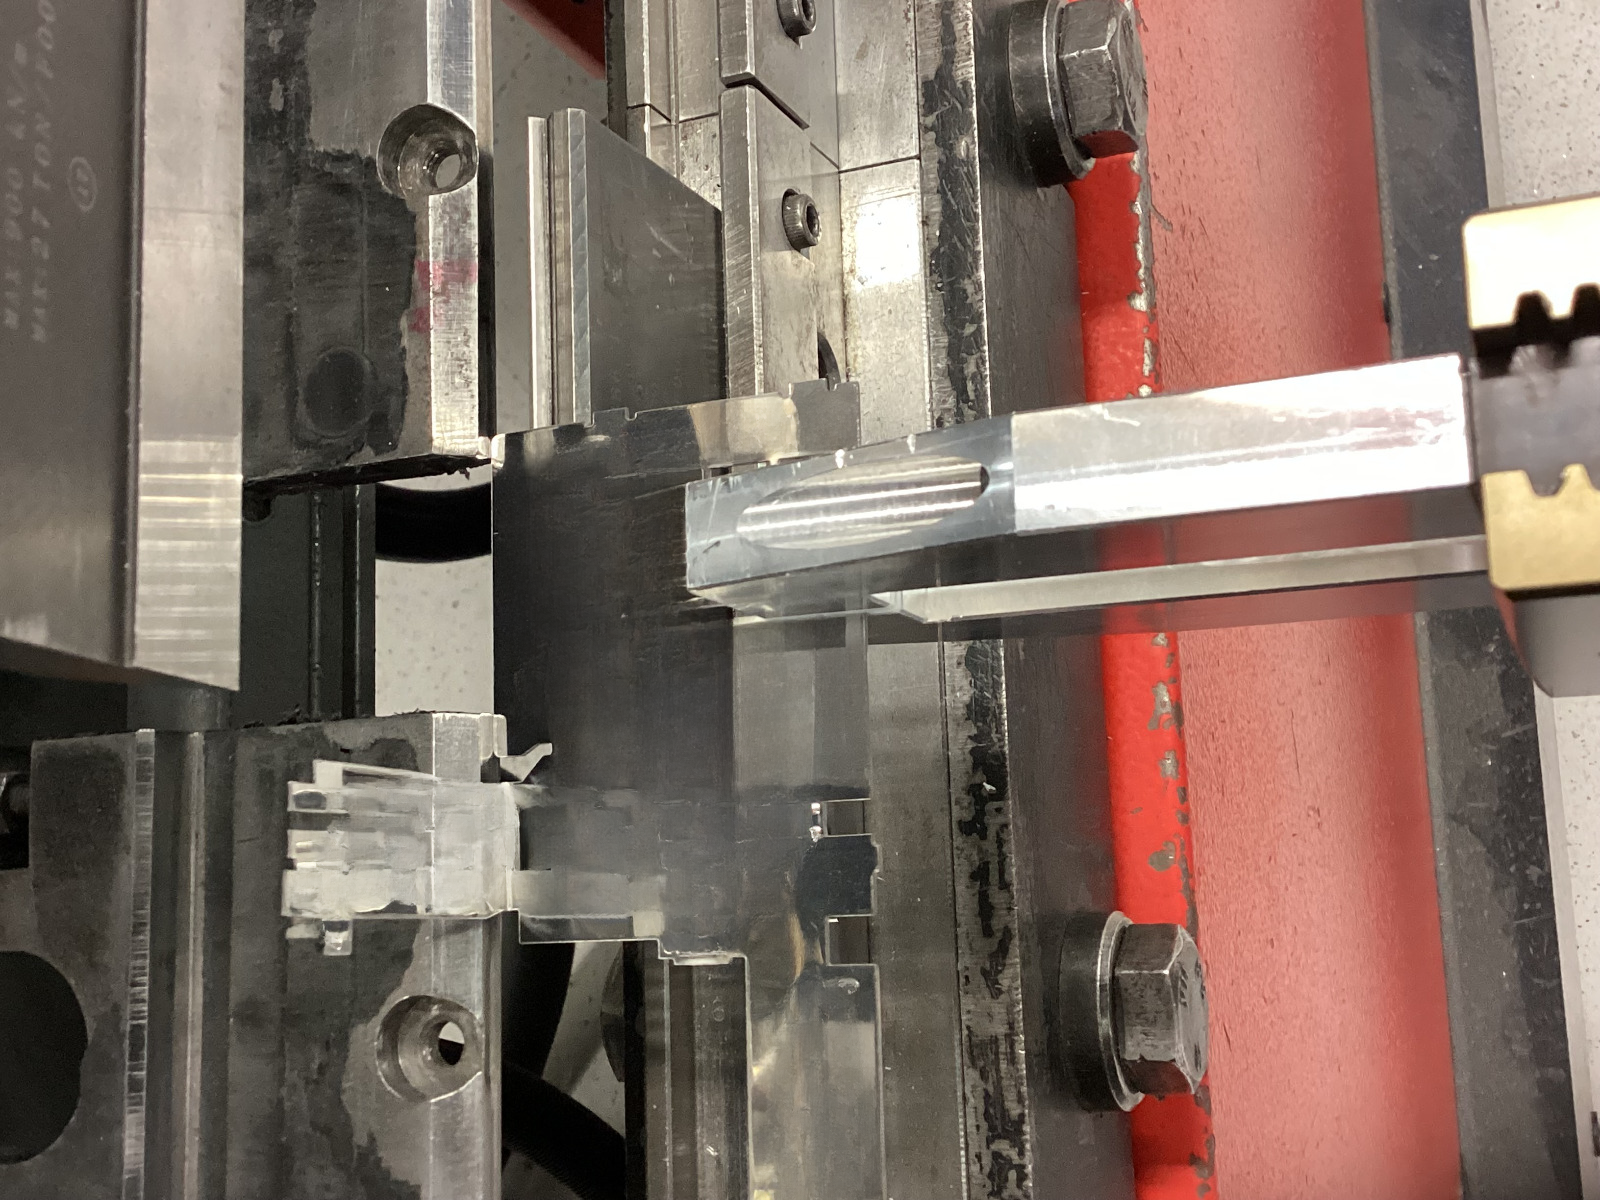
\includegraphics[width=\textwidth]{figures/bending/bending2-003.png}
        \caption{Go to bending station 2}
        \label{subfig:bending2-before}
    \end{subfigure}\hspace{0.1cm}
    \begin{subfigure}[b]{0.32\textwidth}
        \centering
        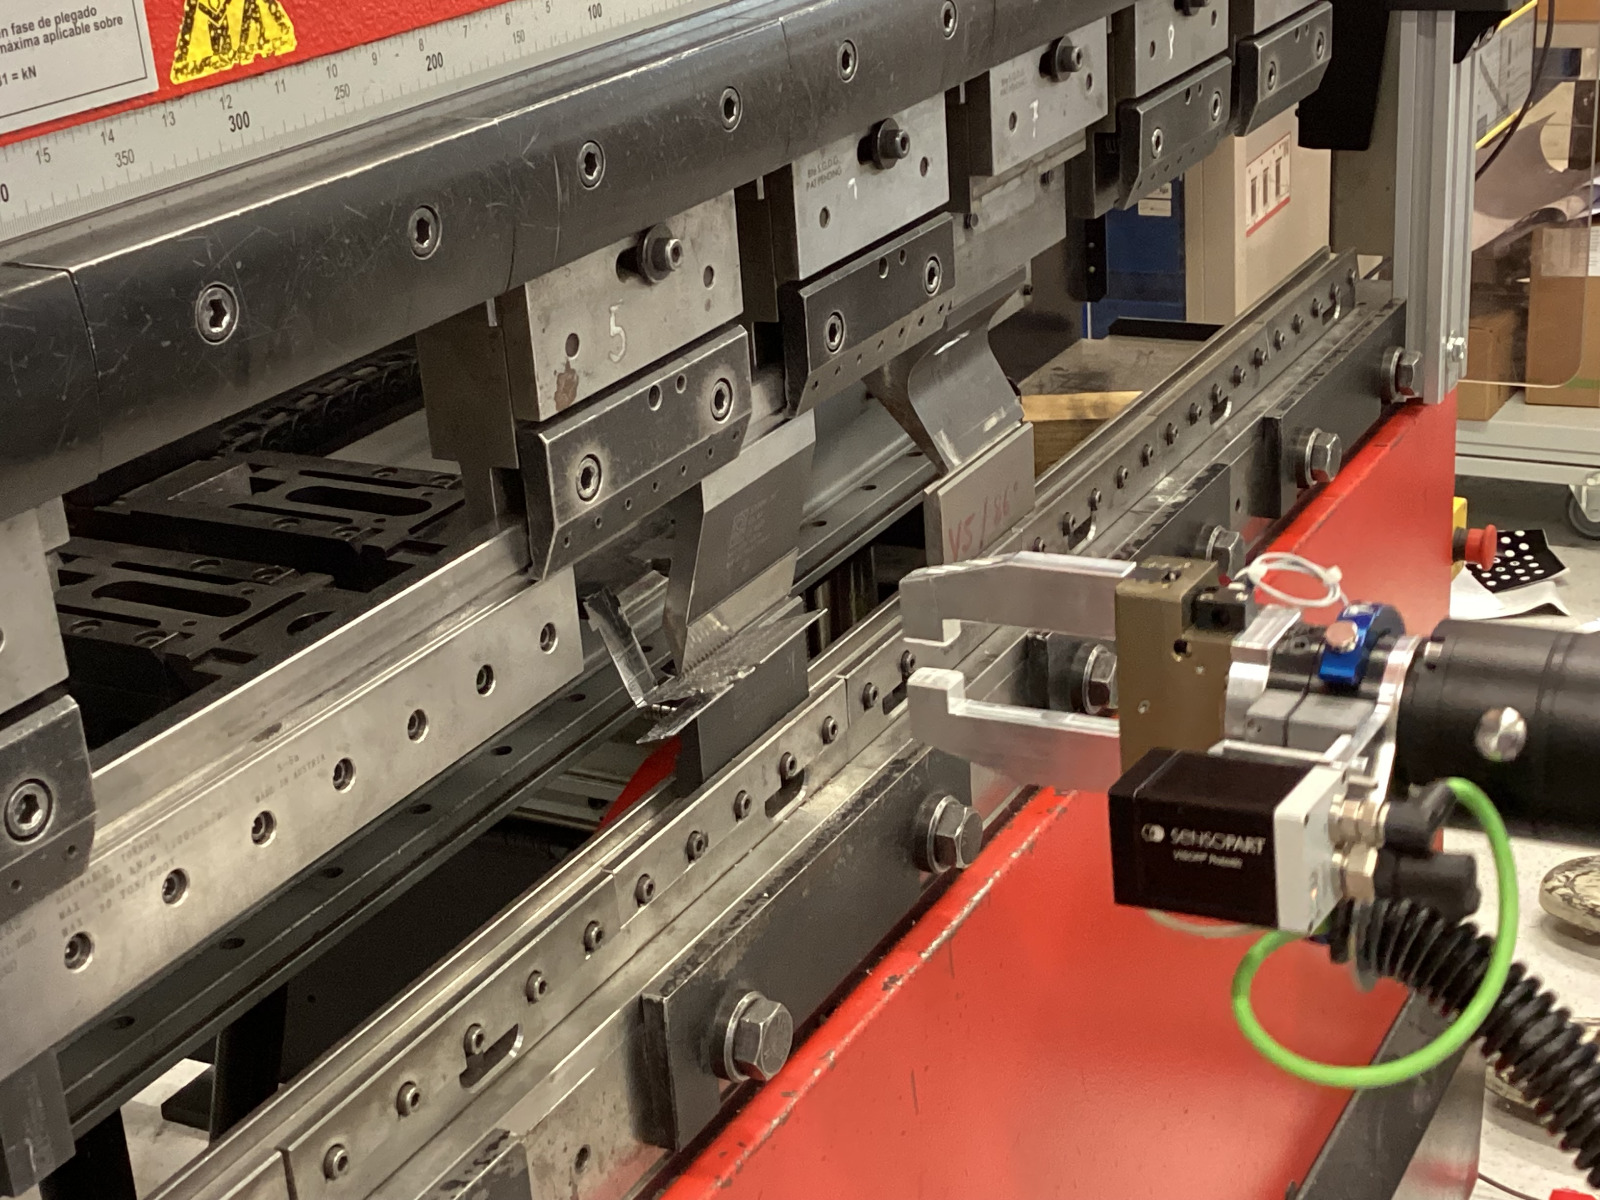
\includegraphics[width=\textwidth]{figures/bending/bending2-001.png}
        \caption{bend the sheet metal part}
        \label{subfig:bending2}
    \end{subfigure}\hspace{0.1cm}
    \begin{subfigure}[b]{0.32\textwidth}
        \centering
        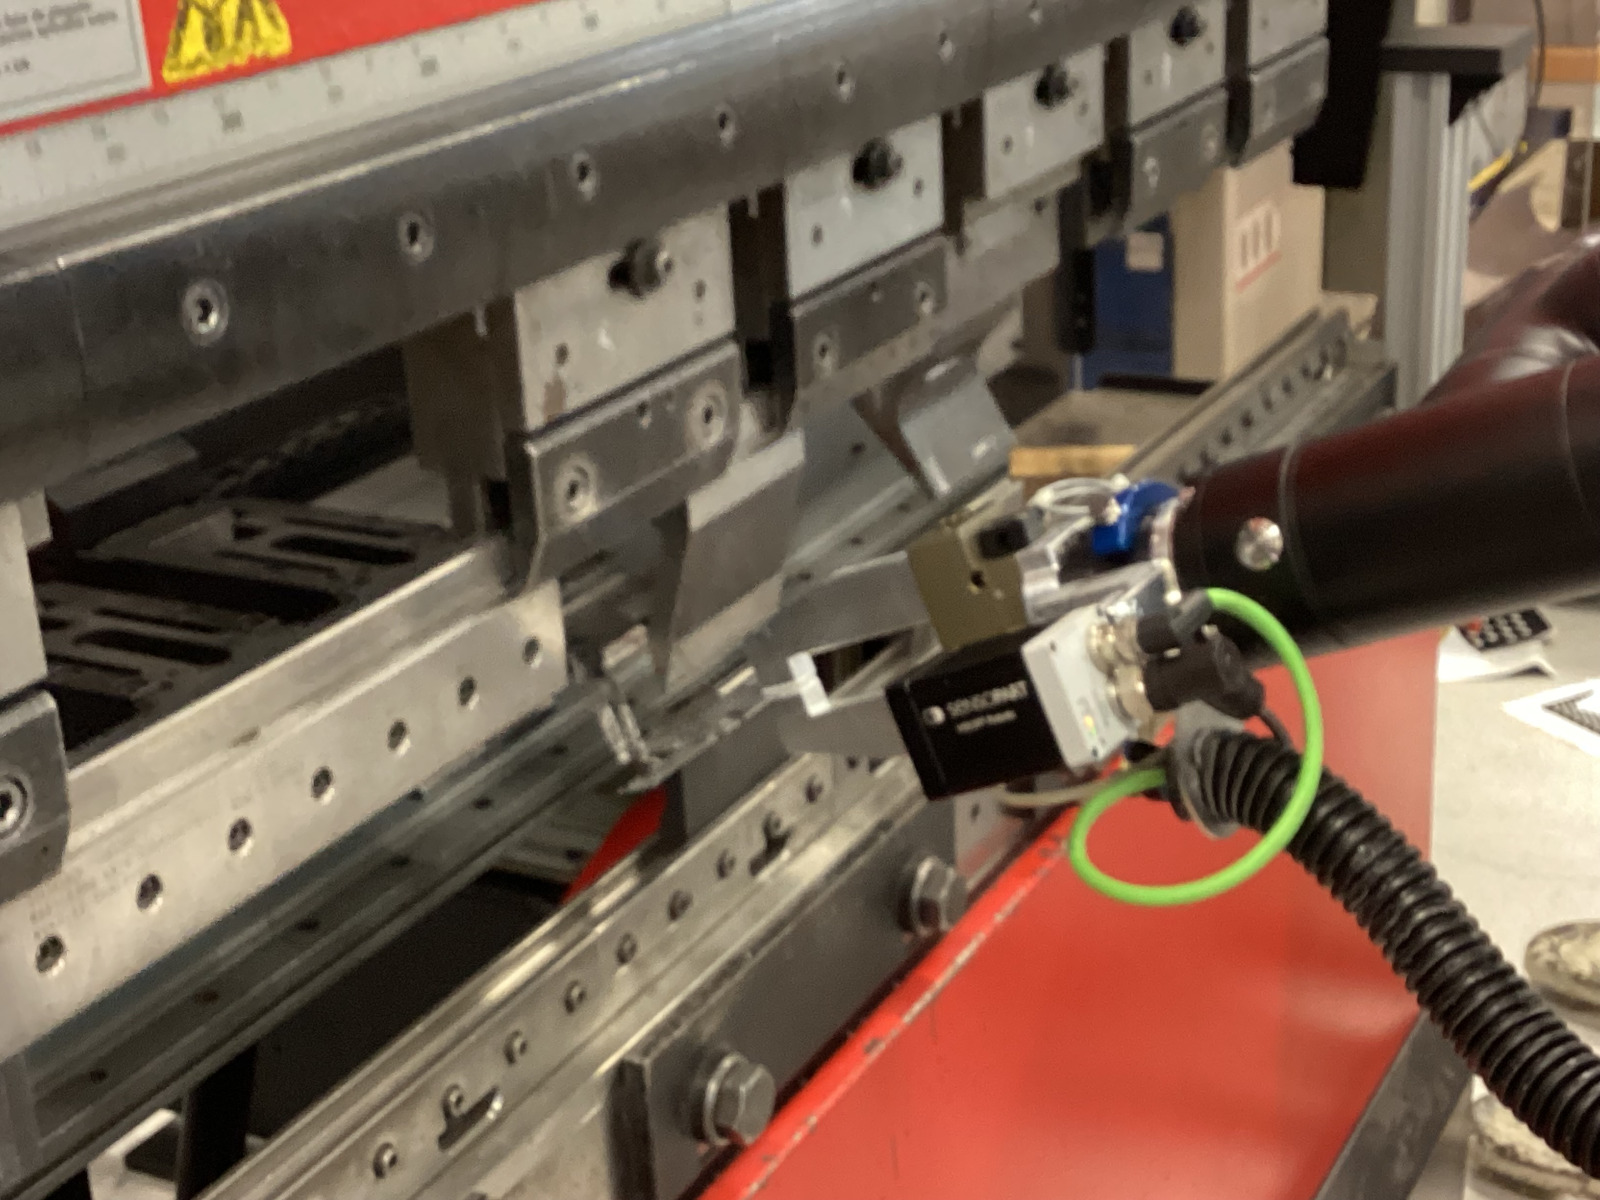
\includegraphics[width=\textwidth]{figures/bending/bending2-002.png}
        \caption{take away the bent sheet}
        \label{subfig:bending2-after}
    \end{subfigure}\hspace{0.1cm}
    \caption{Bending operation number 2 at bending station 2}
    \label{fig:bending-operation-2}
\end{figure}


Figure \ref{fig:bending-operation-1} shows the transfer of sheet metal part to the first bending station where a 90° bend is performed. The handling robot secures the sheet first. A signal is sent by KR1410 robot to PLC to start bending. The robot opens the gripper as soon as the tool of the bending machine hits the sheet. The sheet is secured by the bending machine and the robot moves to a different pose. From there, the robot moves back to the bent part and grip it. Another signal is sent to PLC to move the tool upwards. Once the tool is clear of the part, robot goes to the inspection camera for angle measurement. Bending machine open height measurement laser sensor is responsible for the timings of the opening and closing of bending machine signals. It helps in making robot work together with the bending machine and avoid any collision.


Figures \ref{fig:bending-operation-2} and \ref{fig:bending-operation-3} shows the bending of part at bending station 2. The process is similar to the first bending. The robot leaves the part during bending and regrip it once the bending is complete. For bending number 3, an inspection is not done, because the bending is done very close to the edge, and the small edge is not measurable by the inspection camera.


\begin{figure}[h]
    \centering
    \begin{subfigure}[b]{0.32\textwidth}
        \centering
        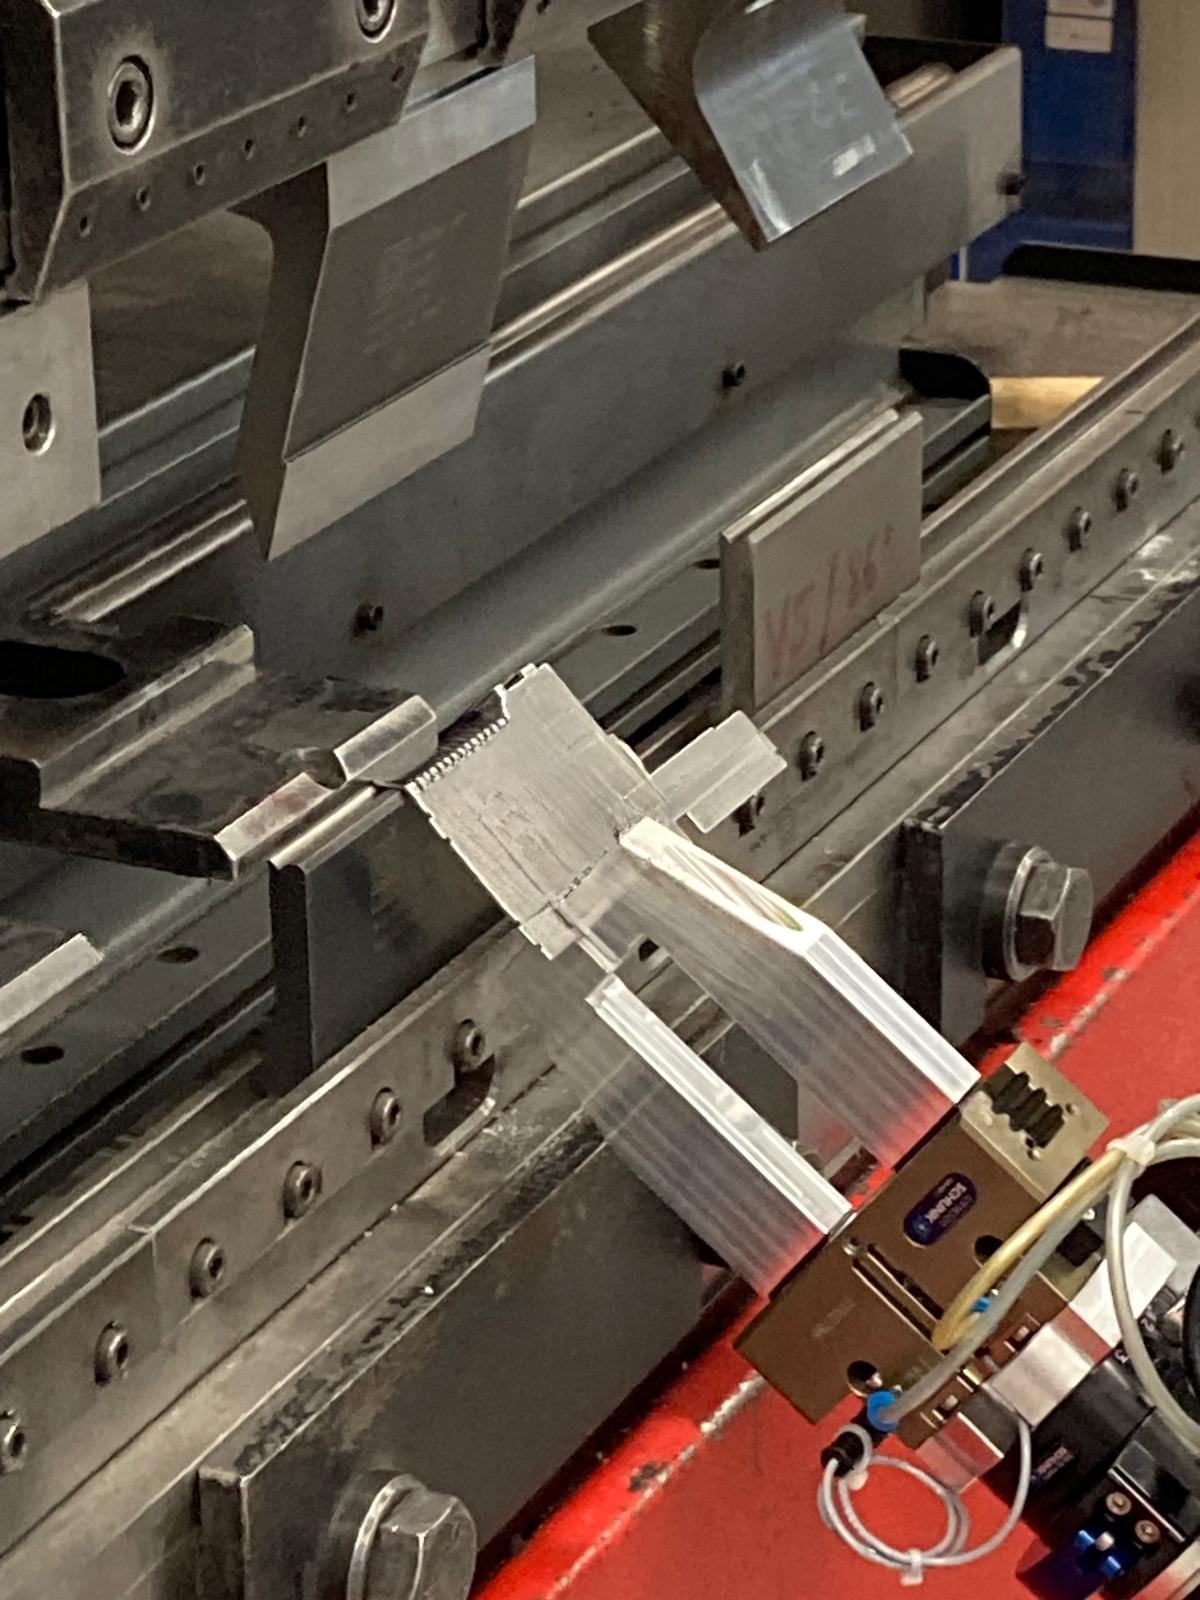
\includegraphics[width=\textwidth]{figures/bending/bending3-001.png}
        \caption{Go to bending station 2}
        \label{subfig:bending3-before}
    \end{subfigure}\hspace{0.1cm}
    \begin{subfigure}[b]{0.32\textwidth}
        \centering
        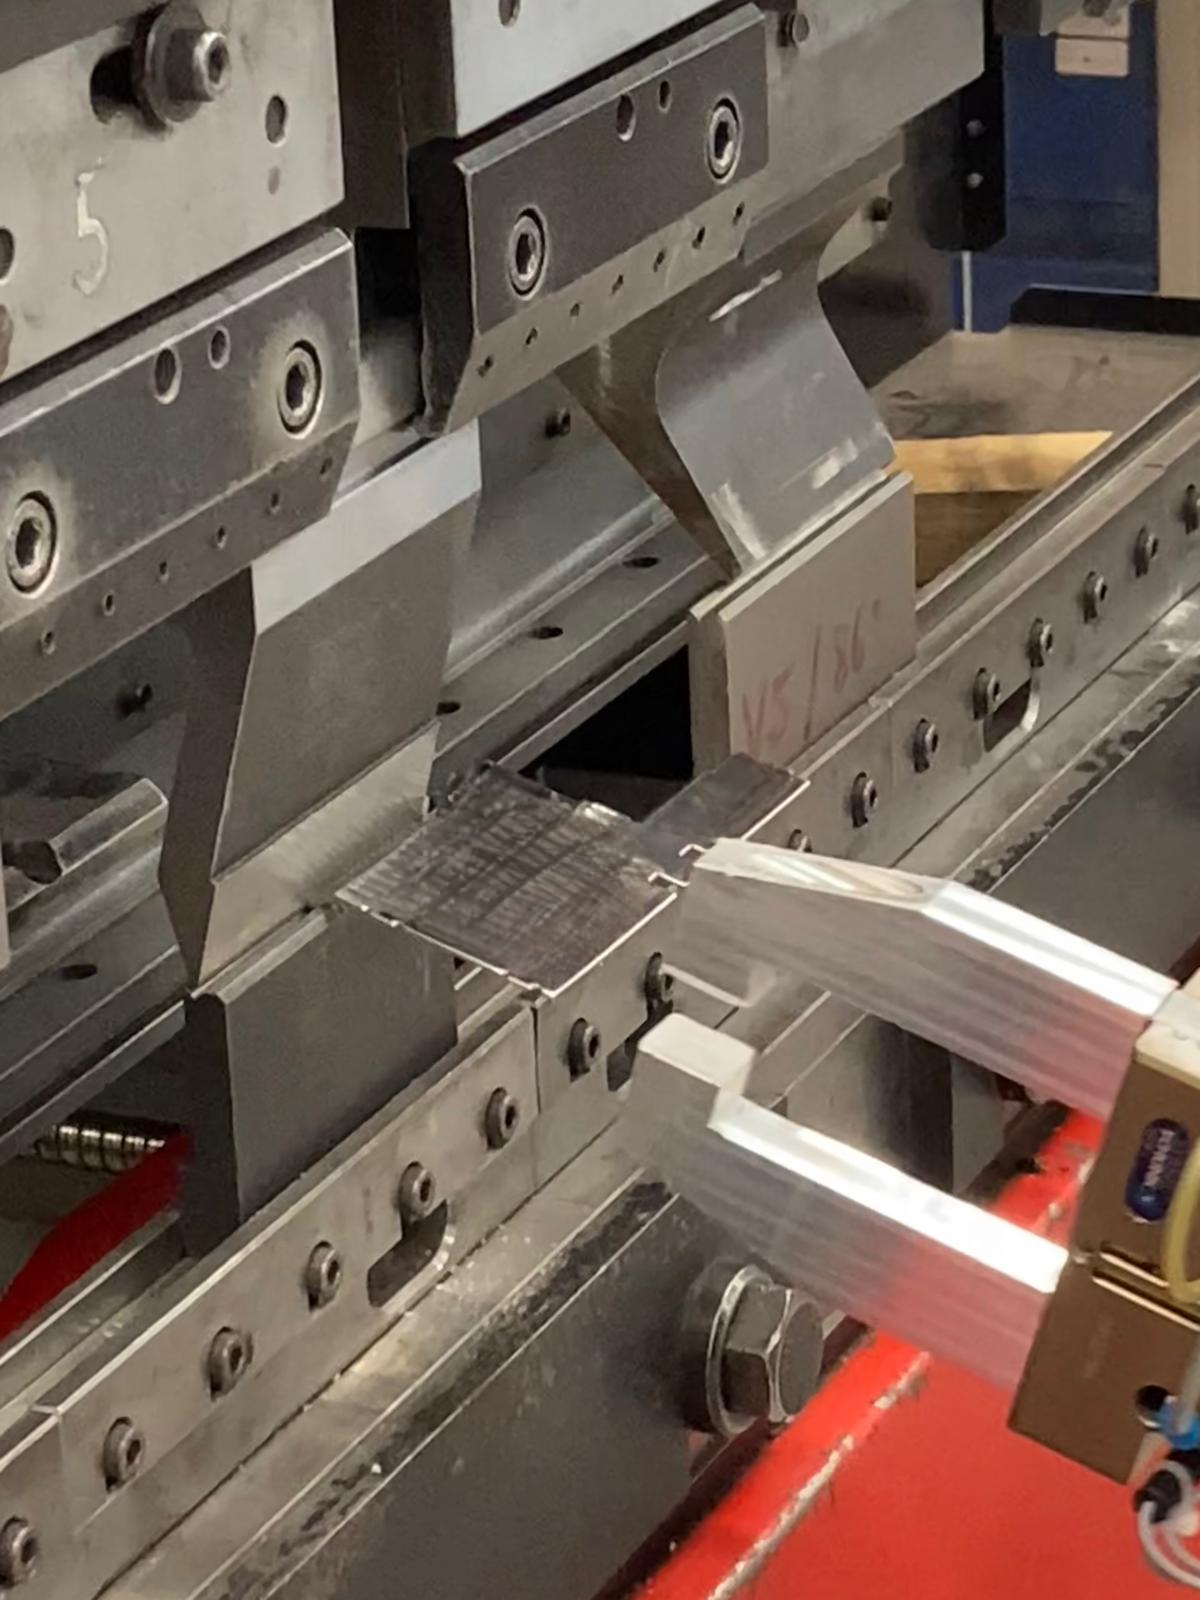
\includegraphics[width=\textwidth]{figures/bending/bending3-002.png}
        \caption{bend the sheet metal part}
        \label{subfig:bending3}
    \end{subfigure}\hspace{0.1cm}
    \begin{subfigure}[b]{0.32\textwidth}
        \centering
        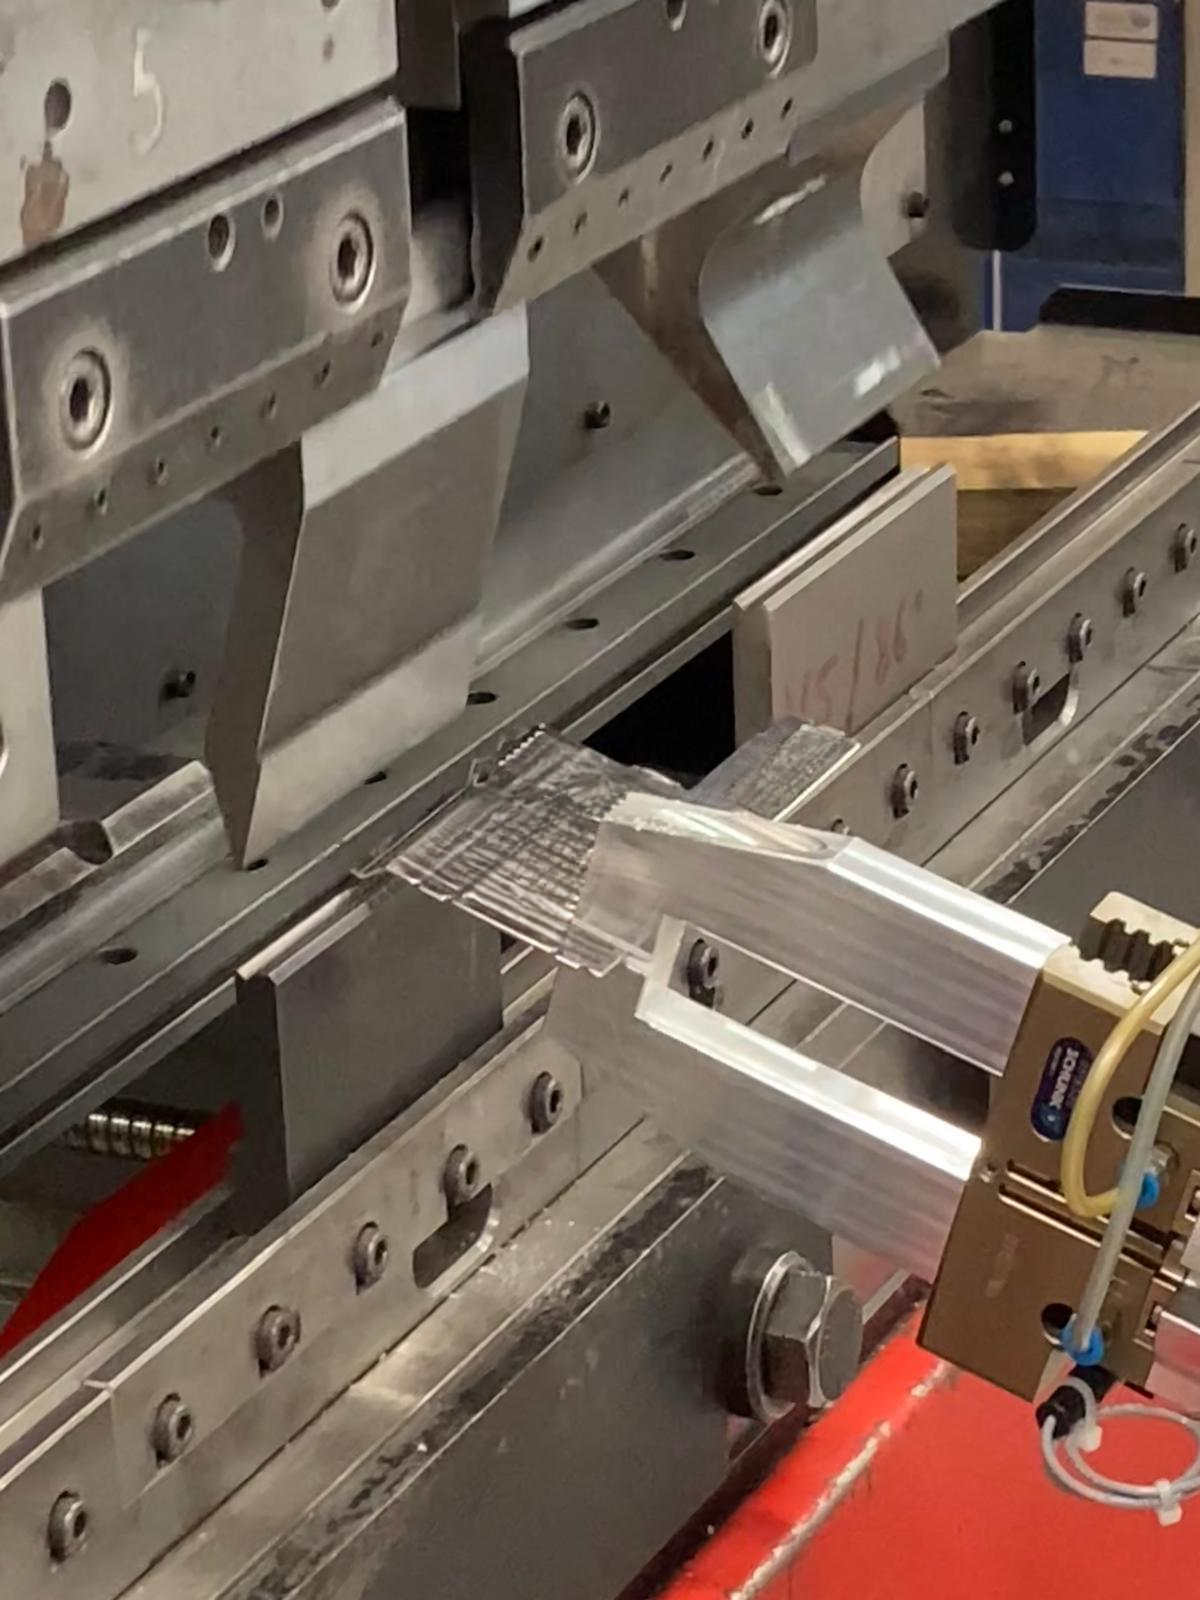
\includegraphics[width=\textwidth]{figures/bending/bending3-003.png}
        \caption{take away the bent sheet}
        \label{subfig:bending3-after}
    \end{subfigure}\hspace{0.1cm}
    \caption{Bending operation number 3 at bending station 2}
    \label{fig:bending-operation-3}
\end{figure}

\begin{figure}[h]
    \centering
    \begin{subfigure}[b]{0.32\textwidth}
        \centering
        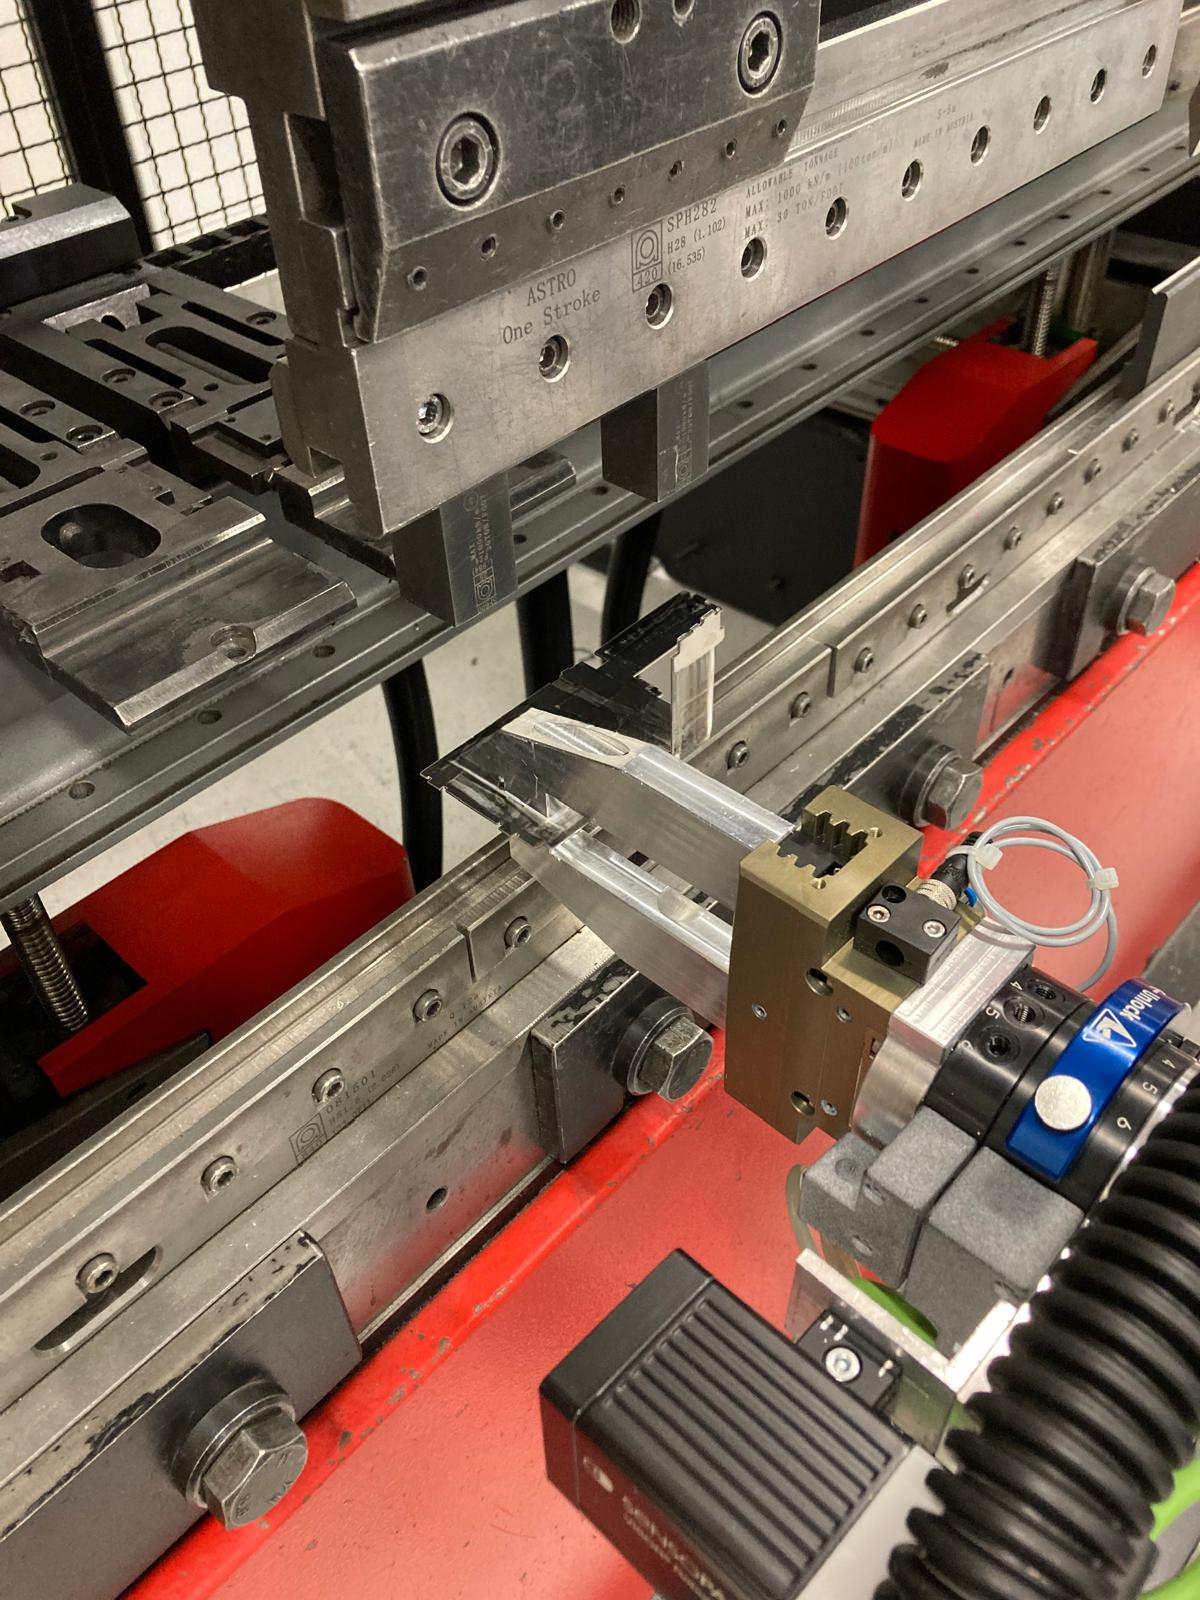
\includegraphics[width=\textwidth]{figures/bending/bending4-001.png}
        \caption{Go to bending station 3}
        \label{subfig:bending4-before}
    \end{subfigure}\hspace{0.1cm}
    \begin{subfigure}[b]{0.32\textwidth}
        \centering
        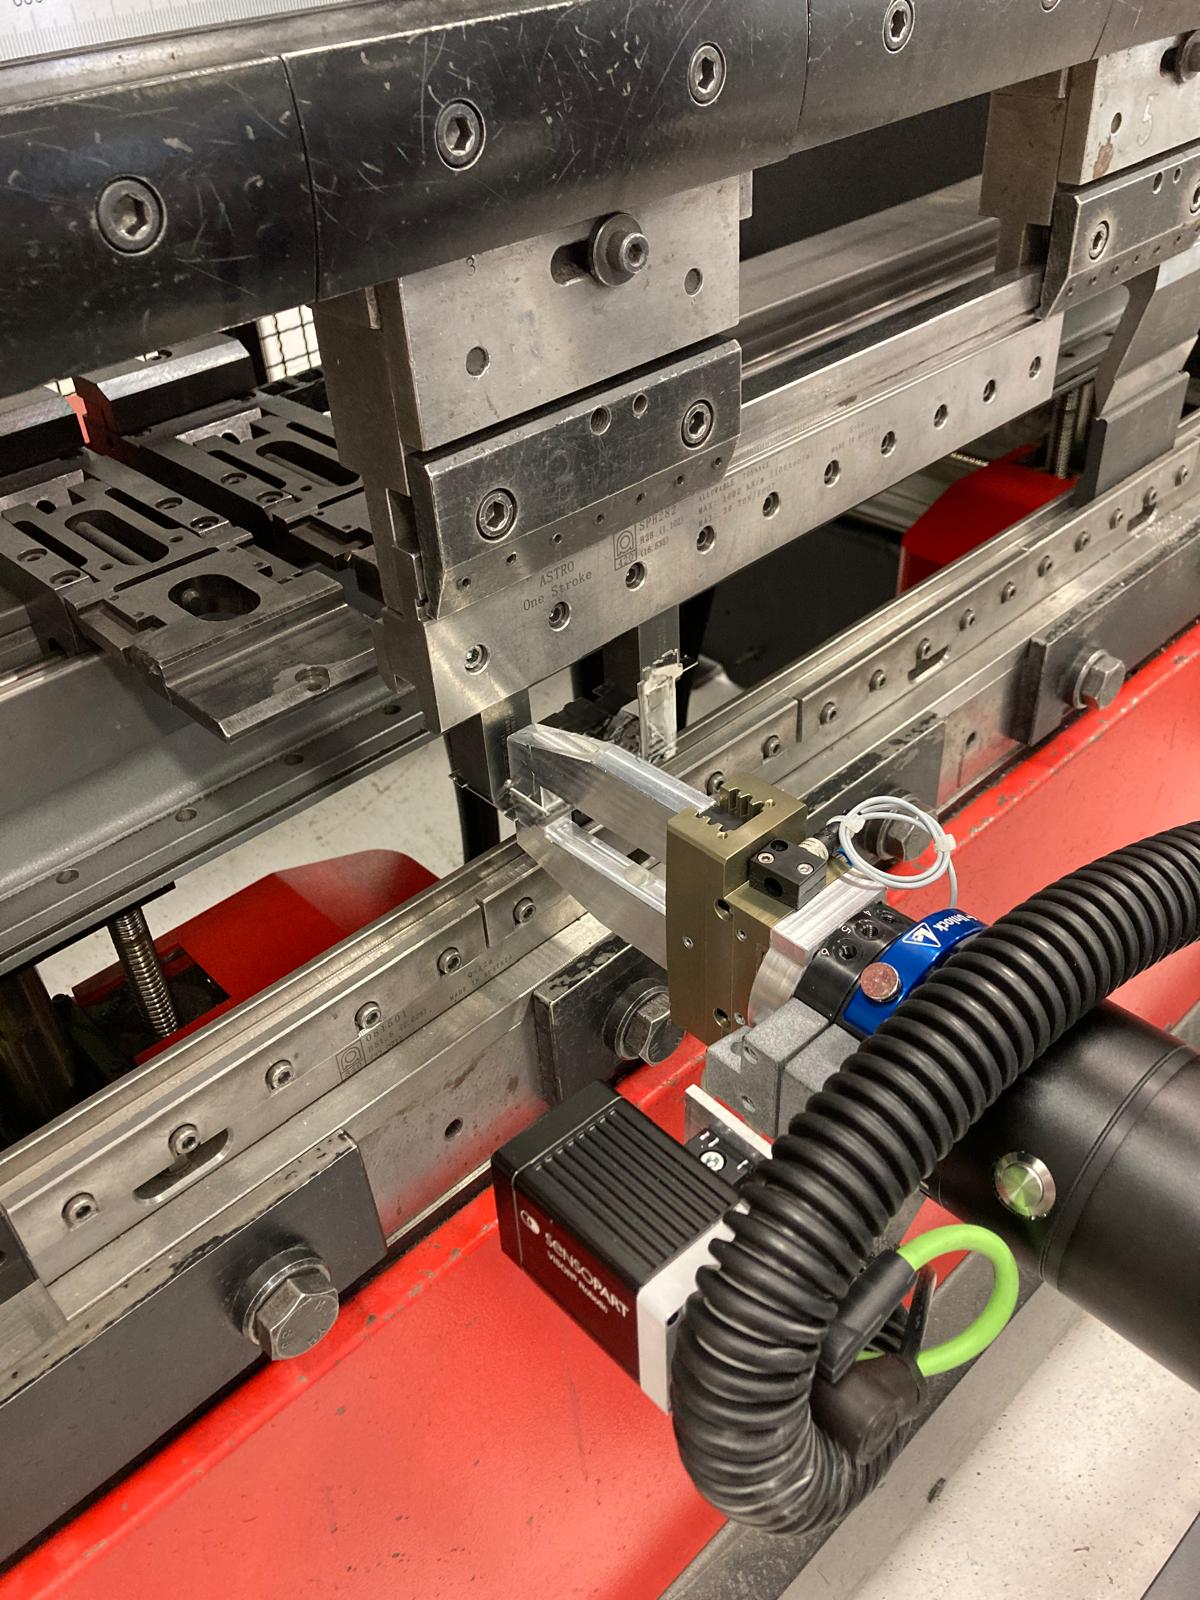
\includegraphics[width=\textwidth]{figures/bending/bending4-002.png}
        \caption{bend the sheet metal part}
        \label{subfig:bending4}
    \end{subfigure}\hspace{0.1cm}
    \begin{subfigure}[b]{0.32\textwidth}
        \centering
        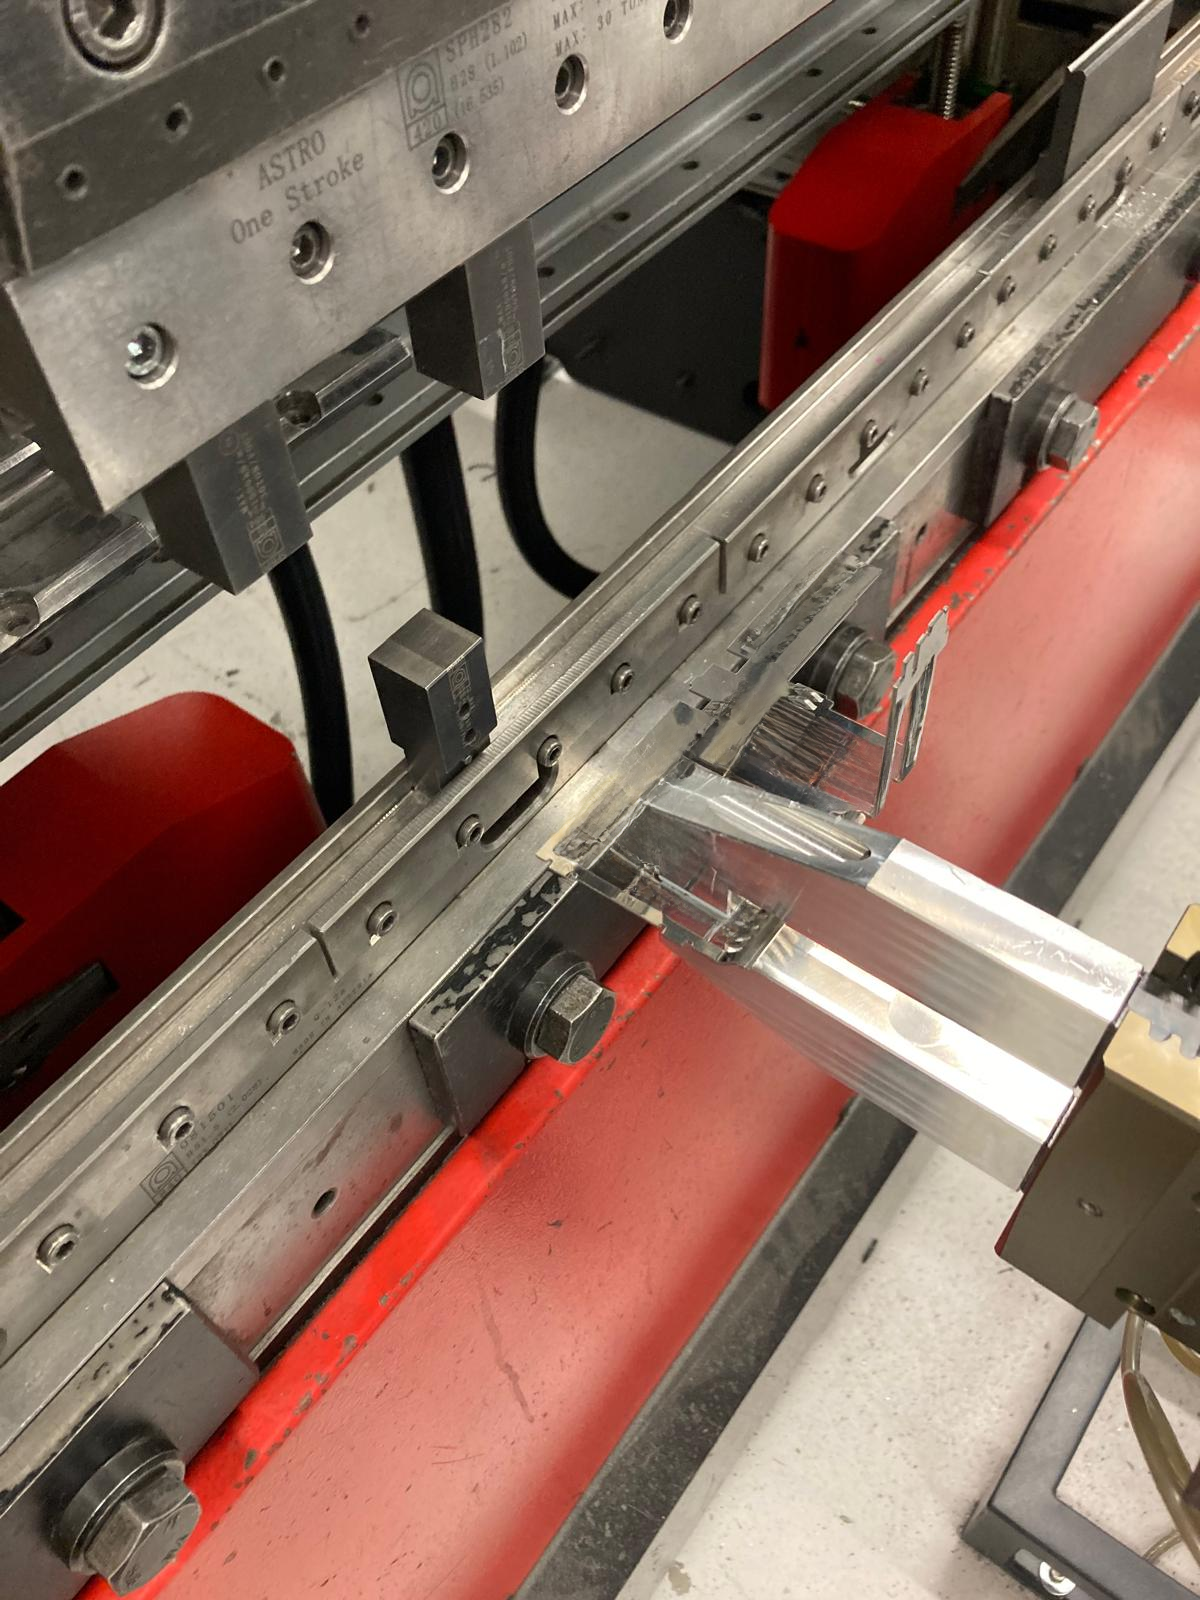
\includegraphics[width=\textwidth]{figures/bending/bending4-003.png}
        \caption{take away the bent sheet}
        \label{subfig:bending4-after}
    \end{subfigure}\hspace{0.1cm}
    \caption{Bending operation number 4 at bending station 3}
    \label{fig:bending-operation-4}
\end{figure}


Figure \ref{fig:bending-operation-4} shows the bending opertion 4 in bending station 3. Since the tool and die are only used for pressing the sheet to flatten it, the robotic gripper doesn't have to open the gripper during bending. Once the sheet is pressed for a specific duration, tool moves up and the robot takes the part out.  Again the inspection is not done, because there is no warping of sheet in this bending operation.


\begin{figure}[h]
    \centering
    \begin{subfigure}[b]{0.32\textwidth}
        \centering
        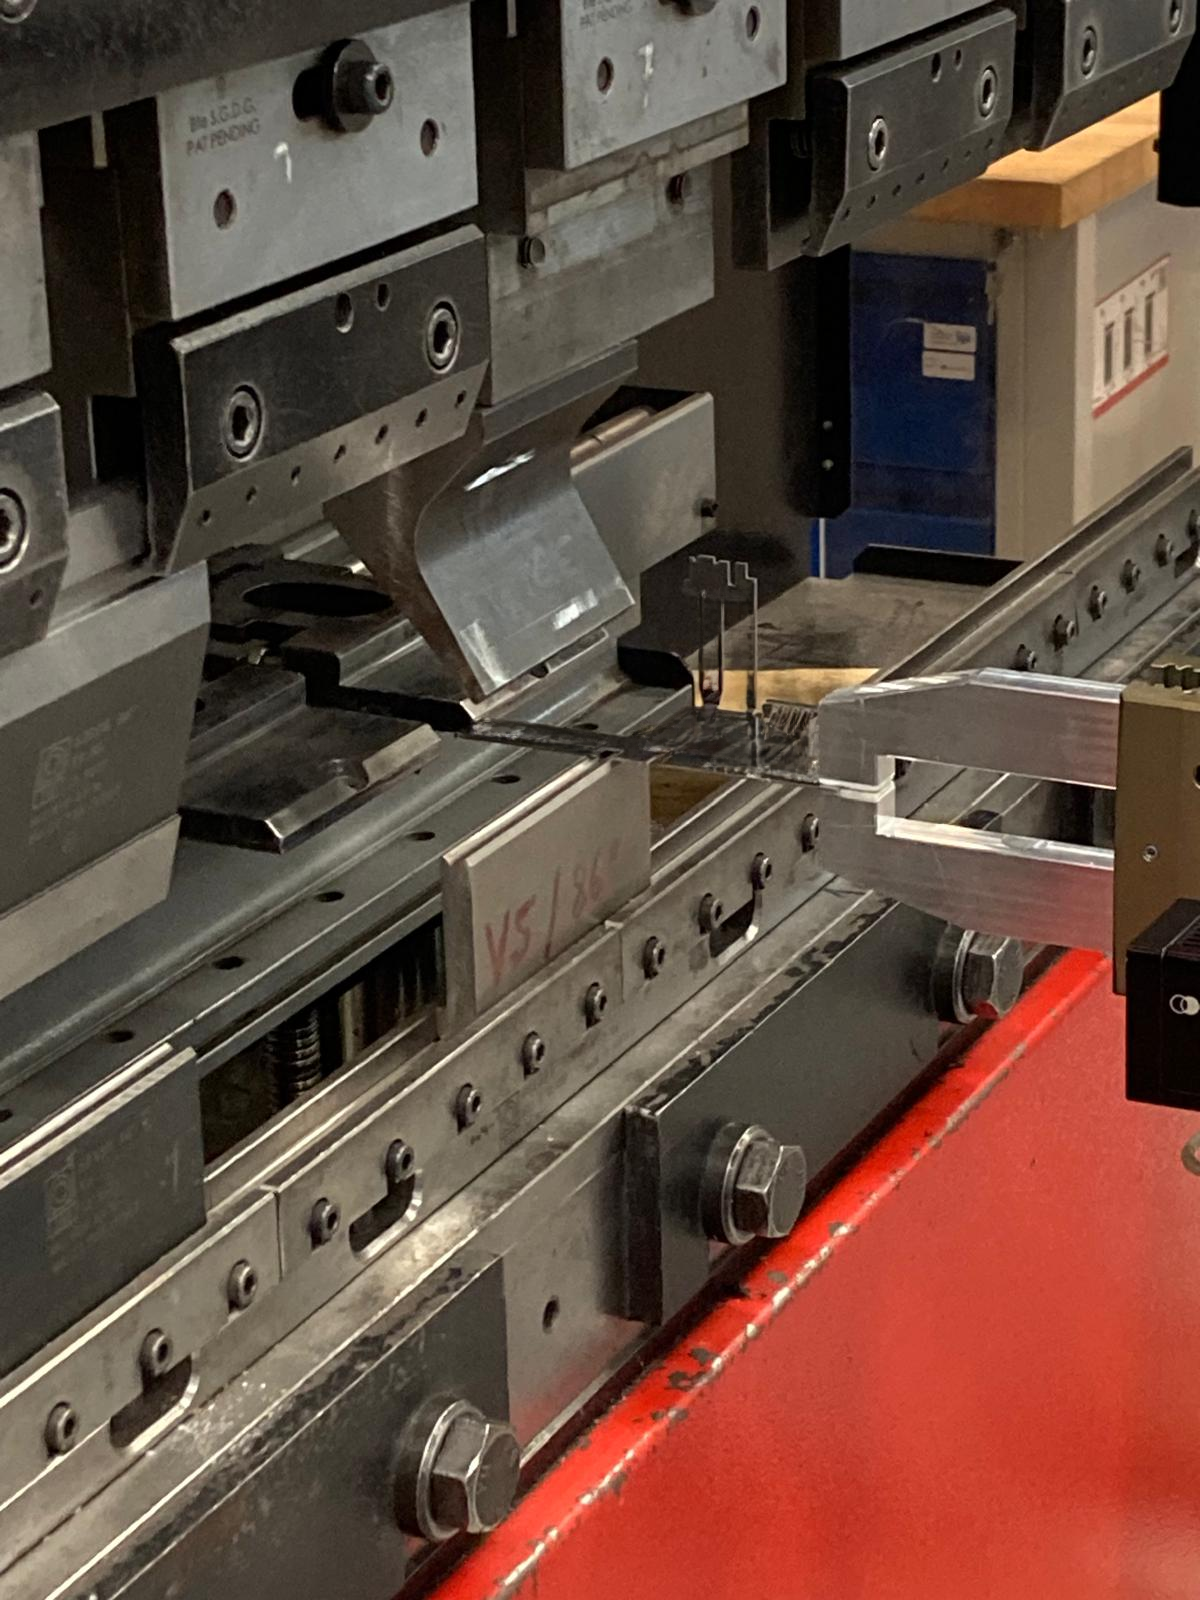
\includegraphics[width=\textwidth]{figures/bending/bending5-001.png}
        \caption{Go to bending station 1}
        \label{subfig:bending5-before}
    \end{subfigure}\hspace{0.1cm}
    \begin{subfigure}[b]{0.32\textwidth}
        \centering
        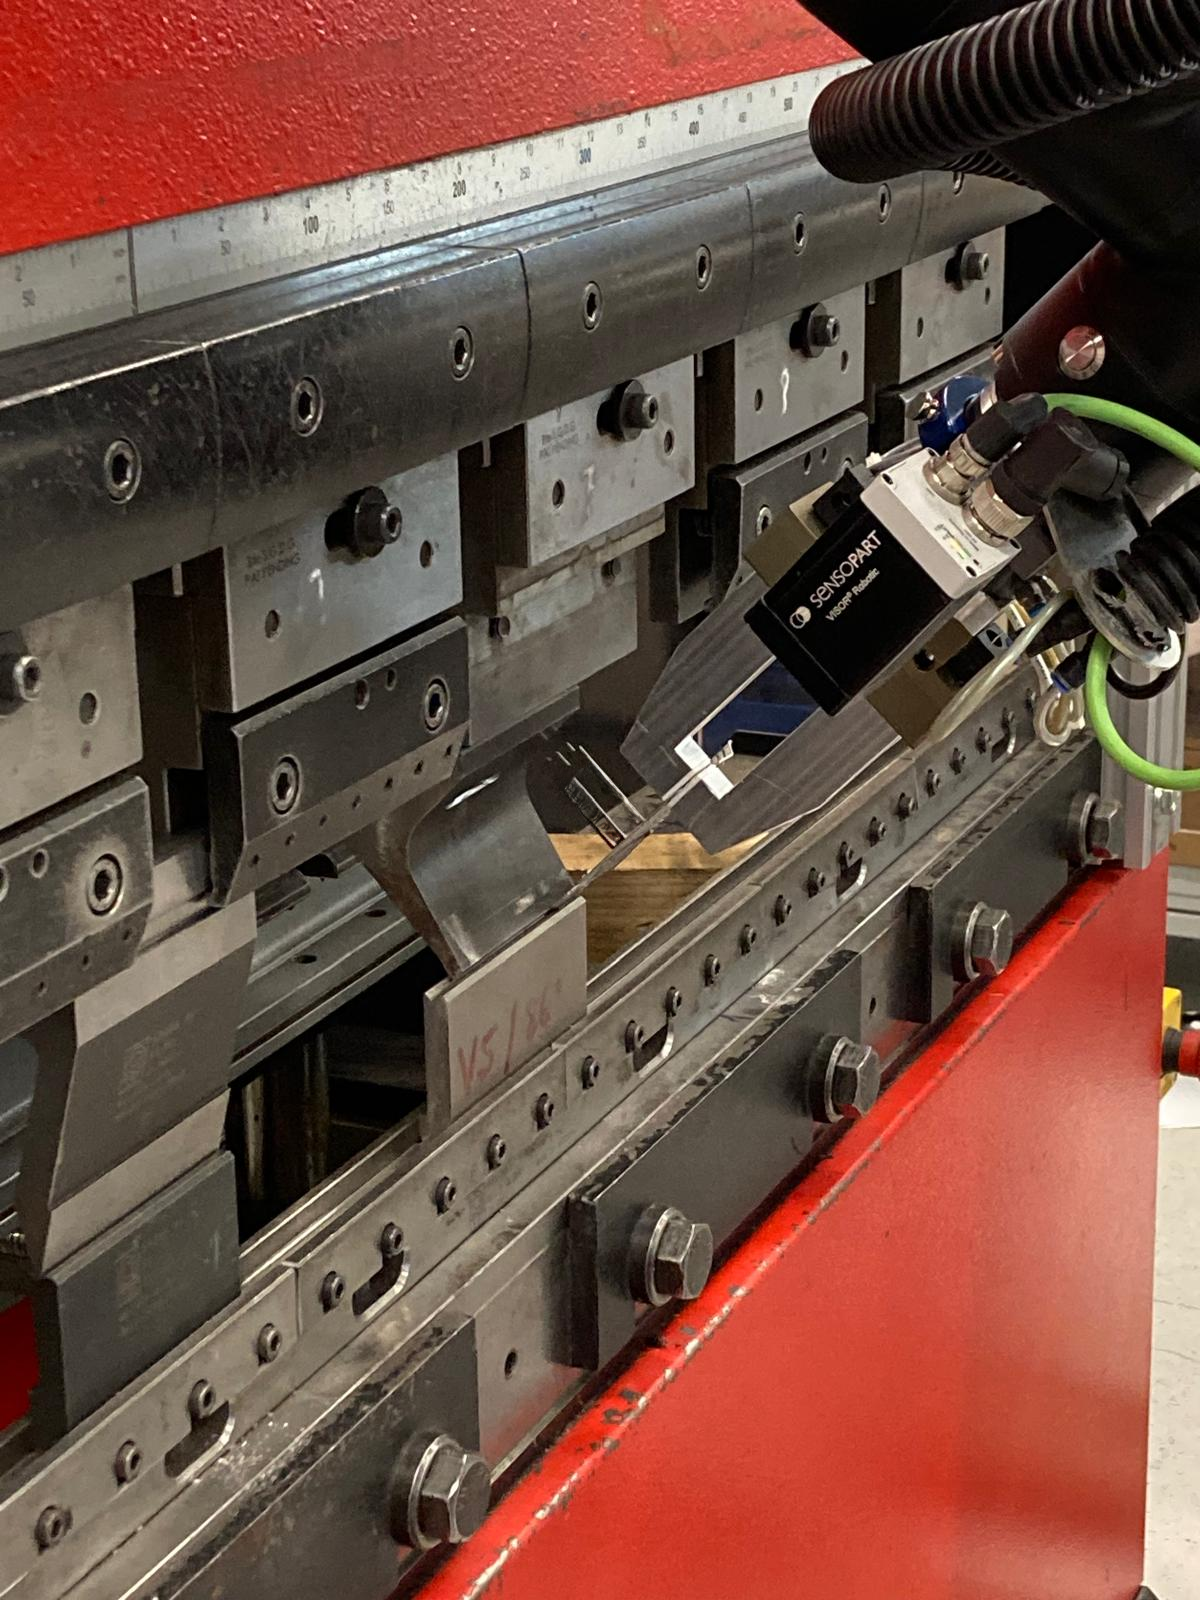
\includegraphics[width=\textwidth]{figures/bending/bending5-002.png}
        \caption{bend the sheet metal part}
        \label{subfig:bending5}
    \end{subfigure}\hspace{0.1cm}
    \begin{subfigure}[b]{0.32\textwidth}
        \centering
        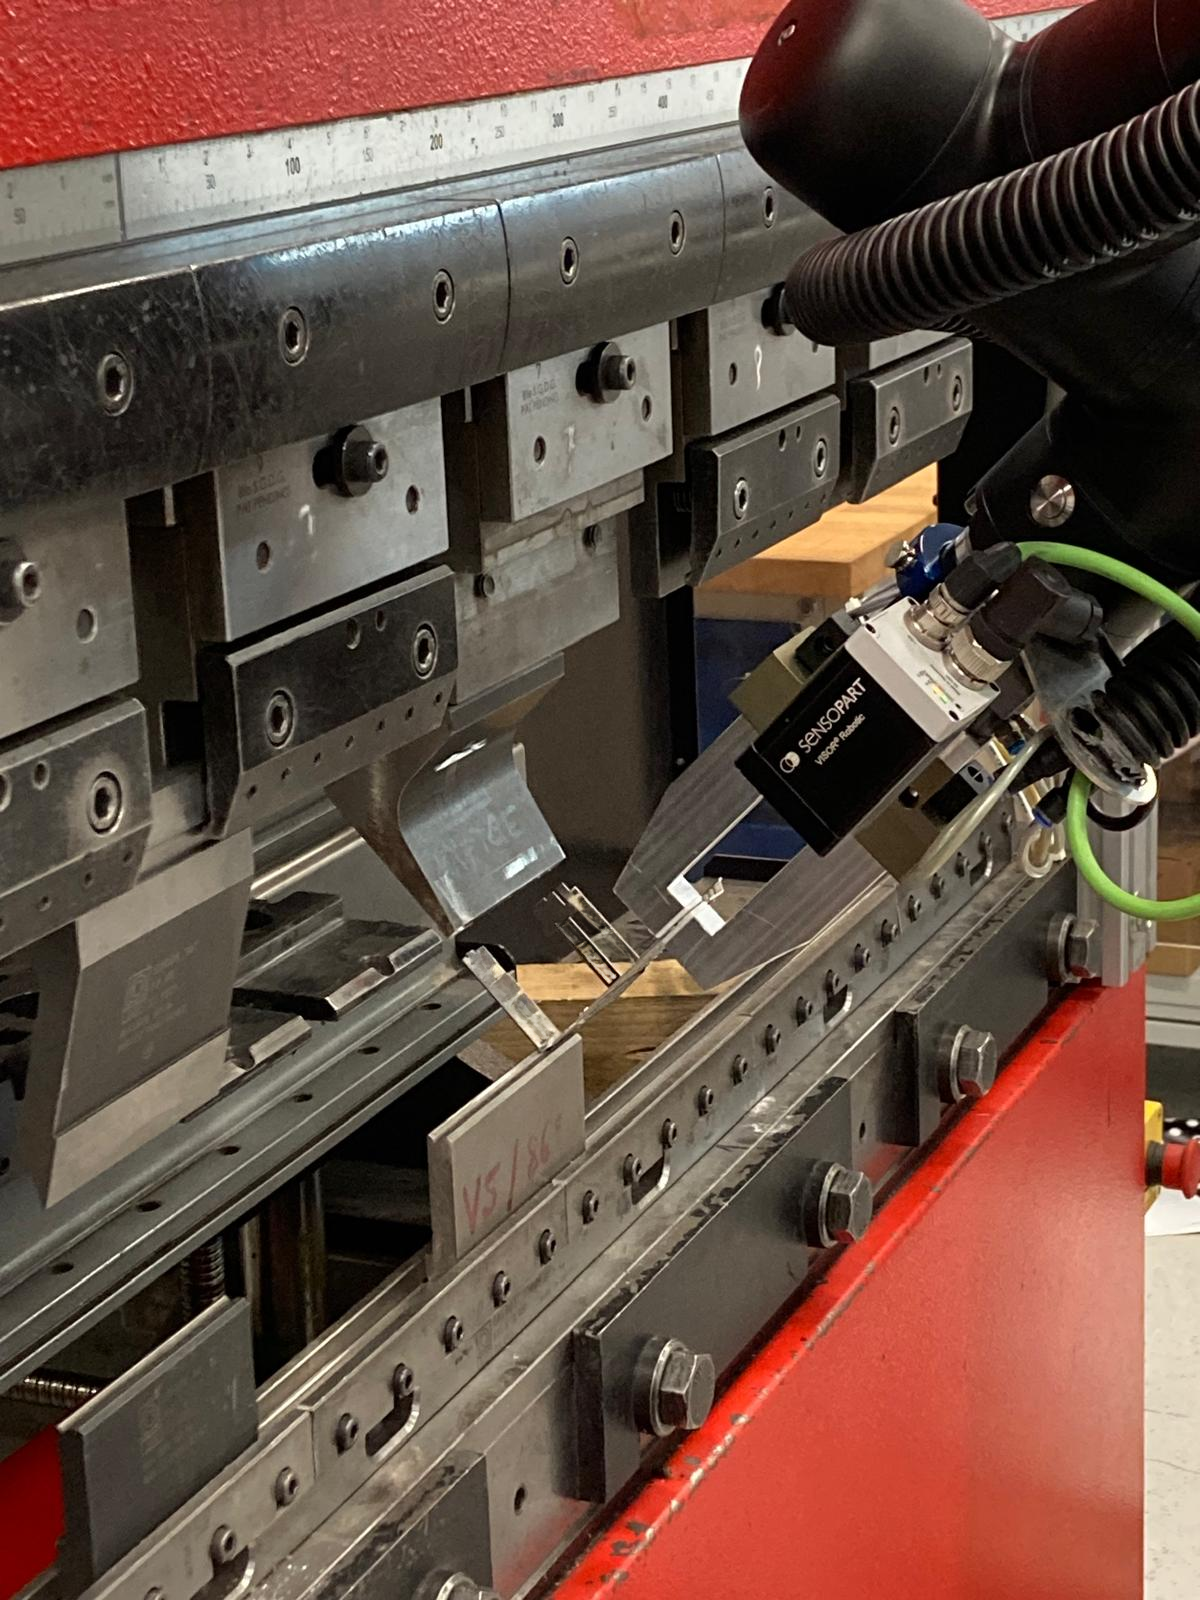
\includegraphics[width=\textwidth]{figures/bending/bending5-003.png}
        \caption{take away the bent sheet}
        \label{subfig:bending5-after}
    \end{subfigure}\hspace{0.1cm}
    \caption{Bending operation number 5 at bending station 1}
    \label{fig:bending-operation-5}
\end{figure}


\begin{figure}[h]
    \centering
    \begin{subfigure}[b]{0.32\textwidth}
        \centering
        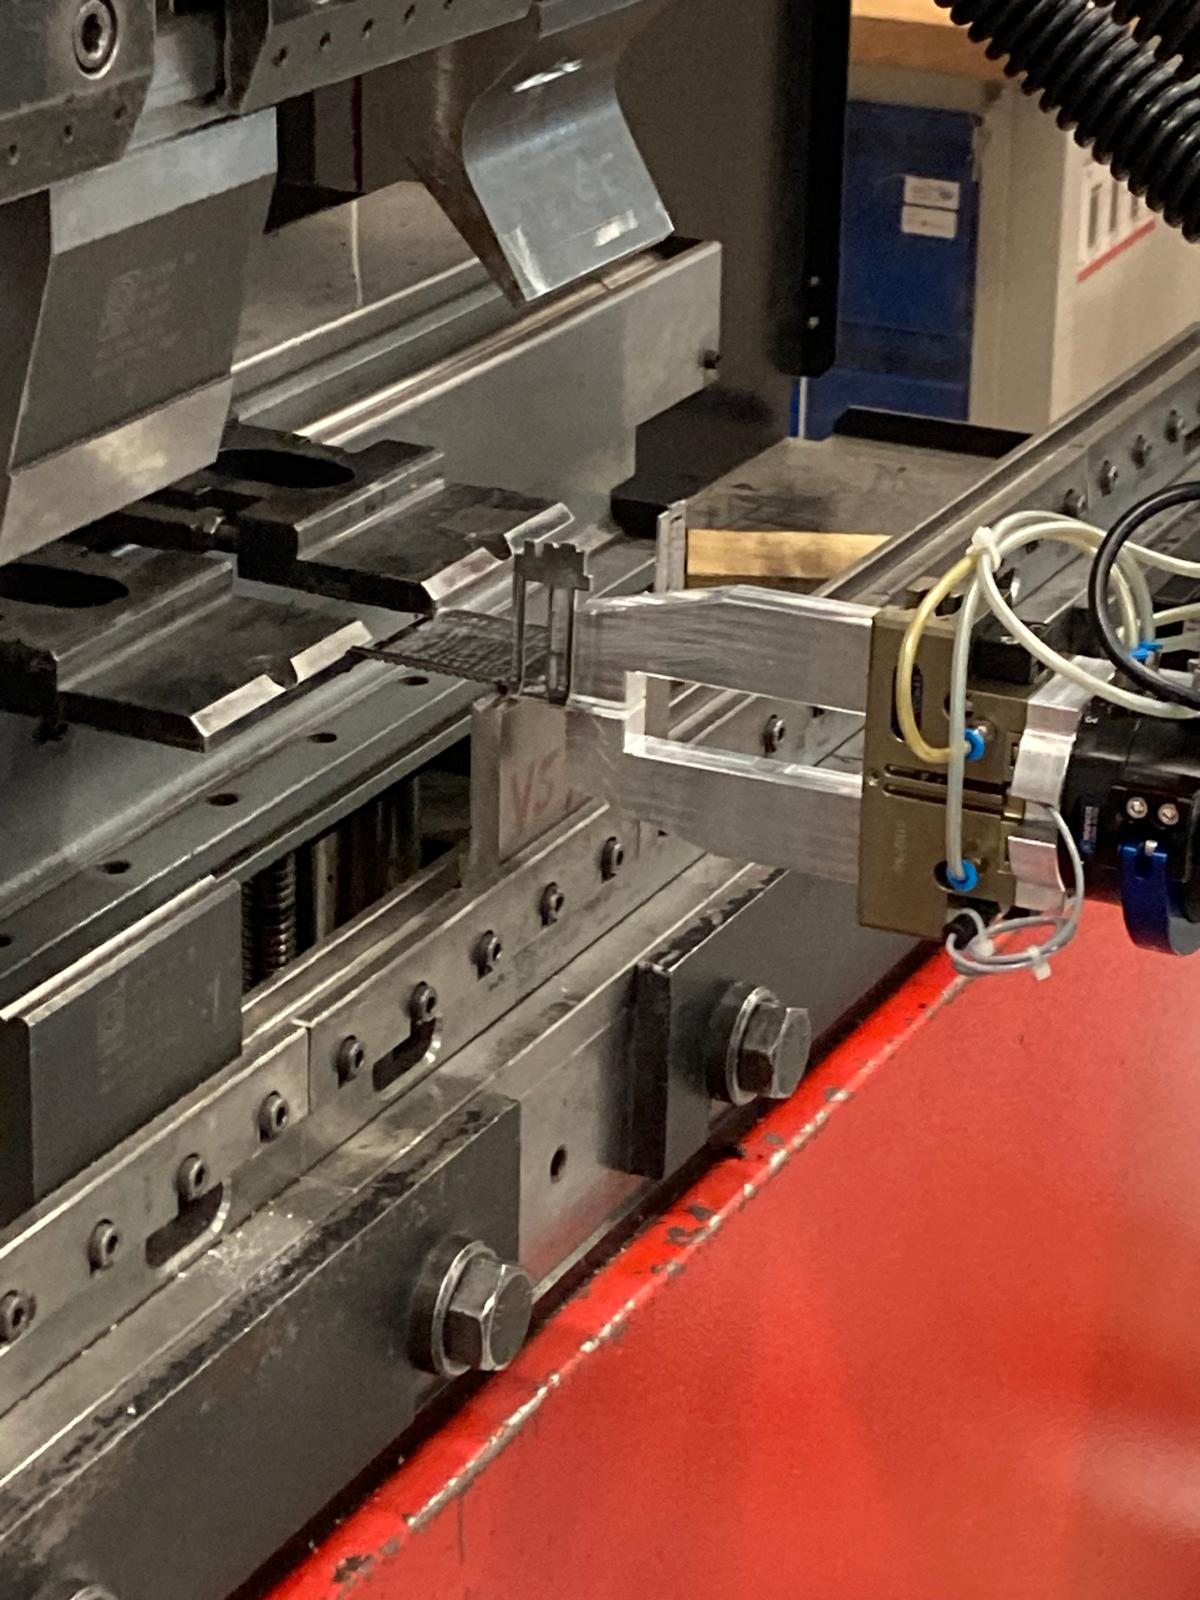
\includegraphics[width=\textwidth]{figures/bending/bending6-001.png}
        \caption{Go to bending station 1}
        \label{subfig:bending6-before}
    \end{subfigure}\hspace{0.1cm}
    \begin{subfigure}[b]{0.32\textwidth}
        \centering
        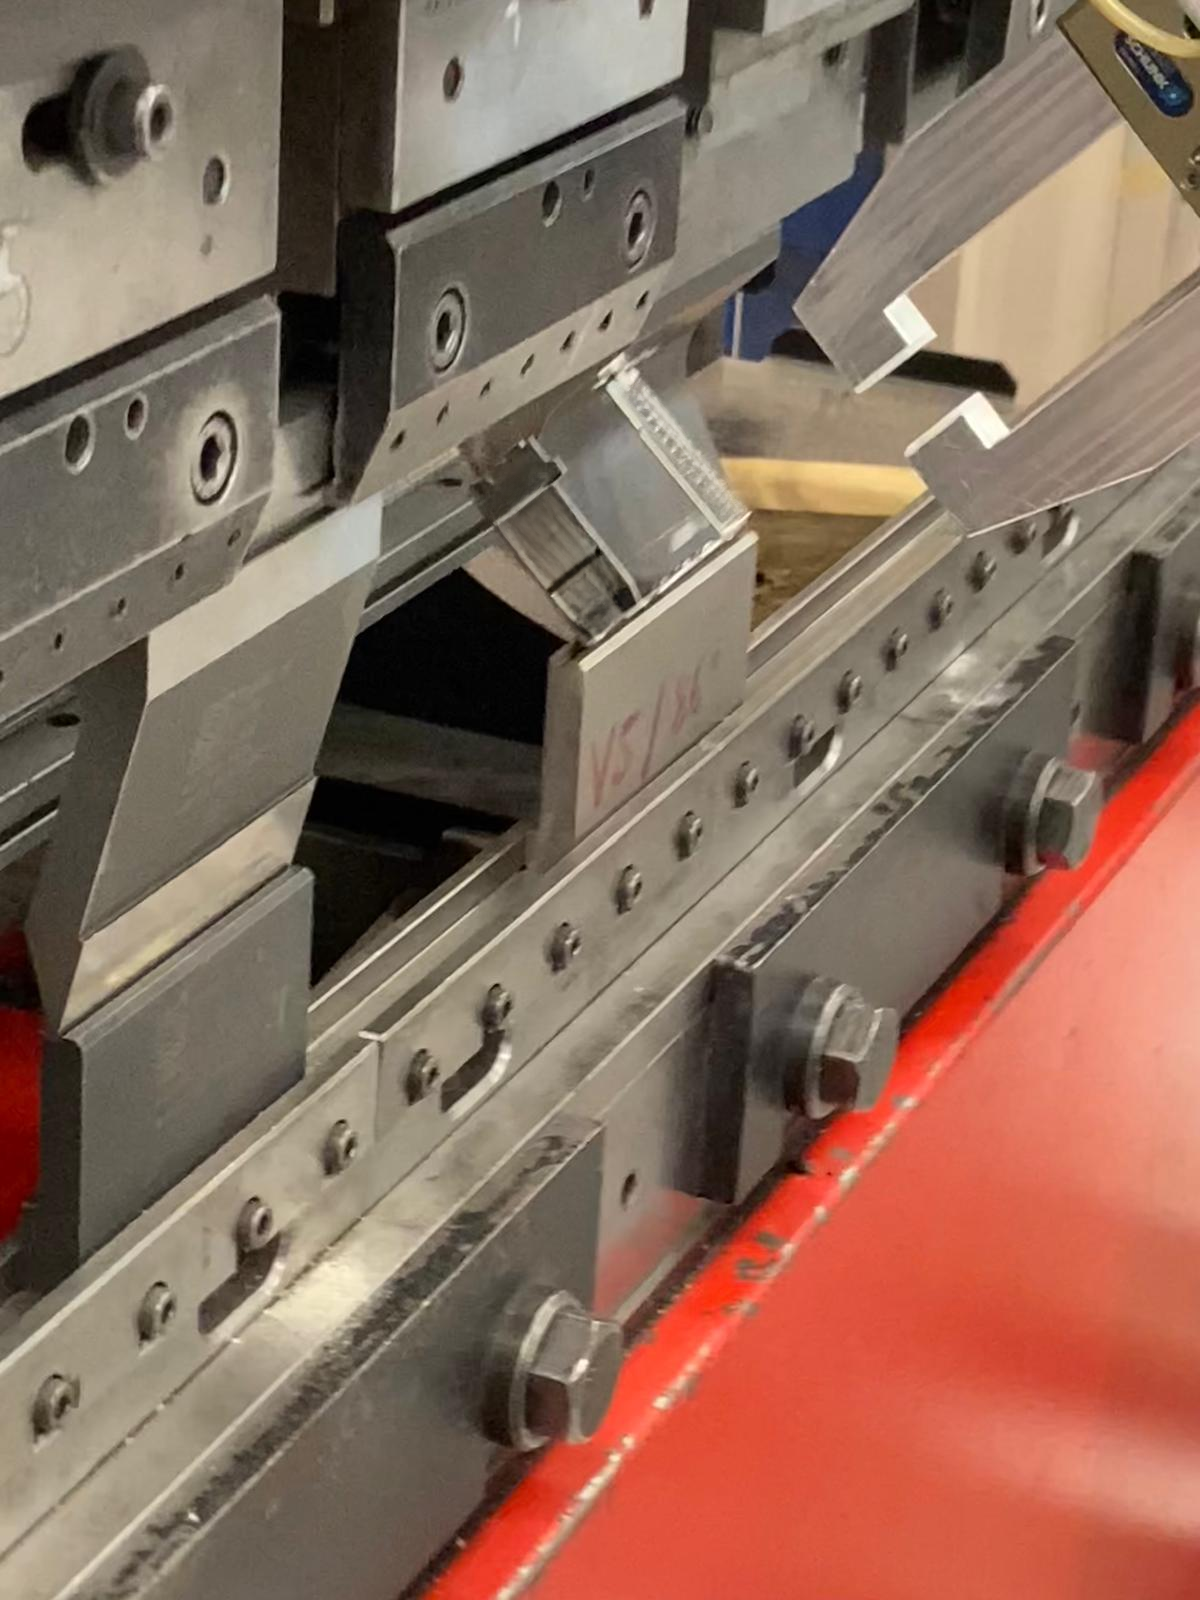
\includegraphics[width=\textwidth]{figures/bending/bending6-003.png}
        \caption{bend the sheet metal part}
        \label{subfig:bending6}
    \end{subfigure}\hspace{0.1cm}
    \begin{subfigure}[b]{0.32\textwidth}
        \centering
        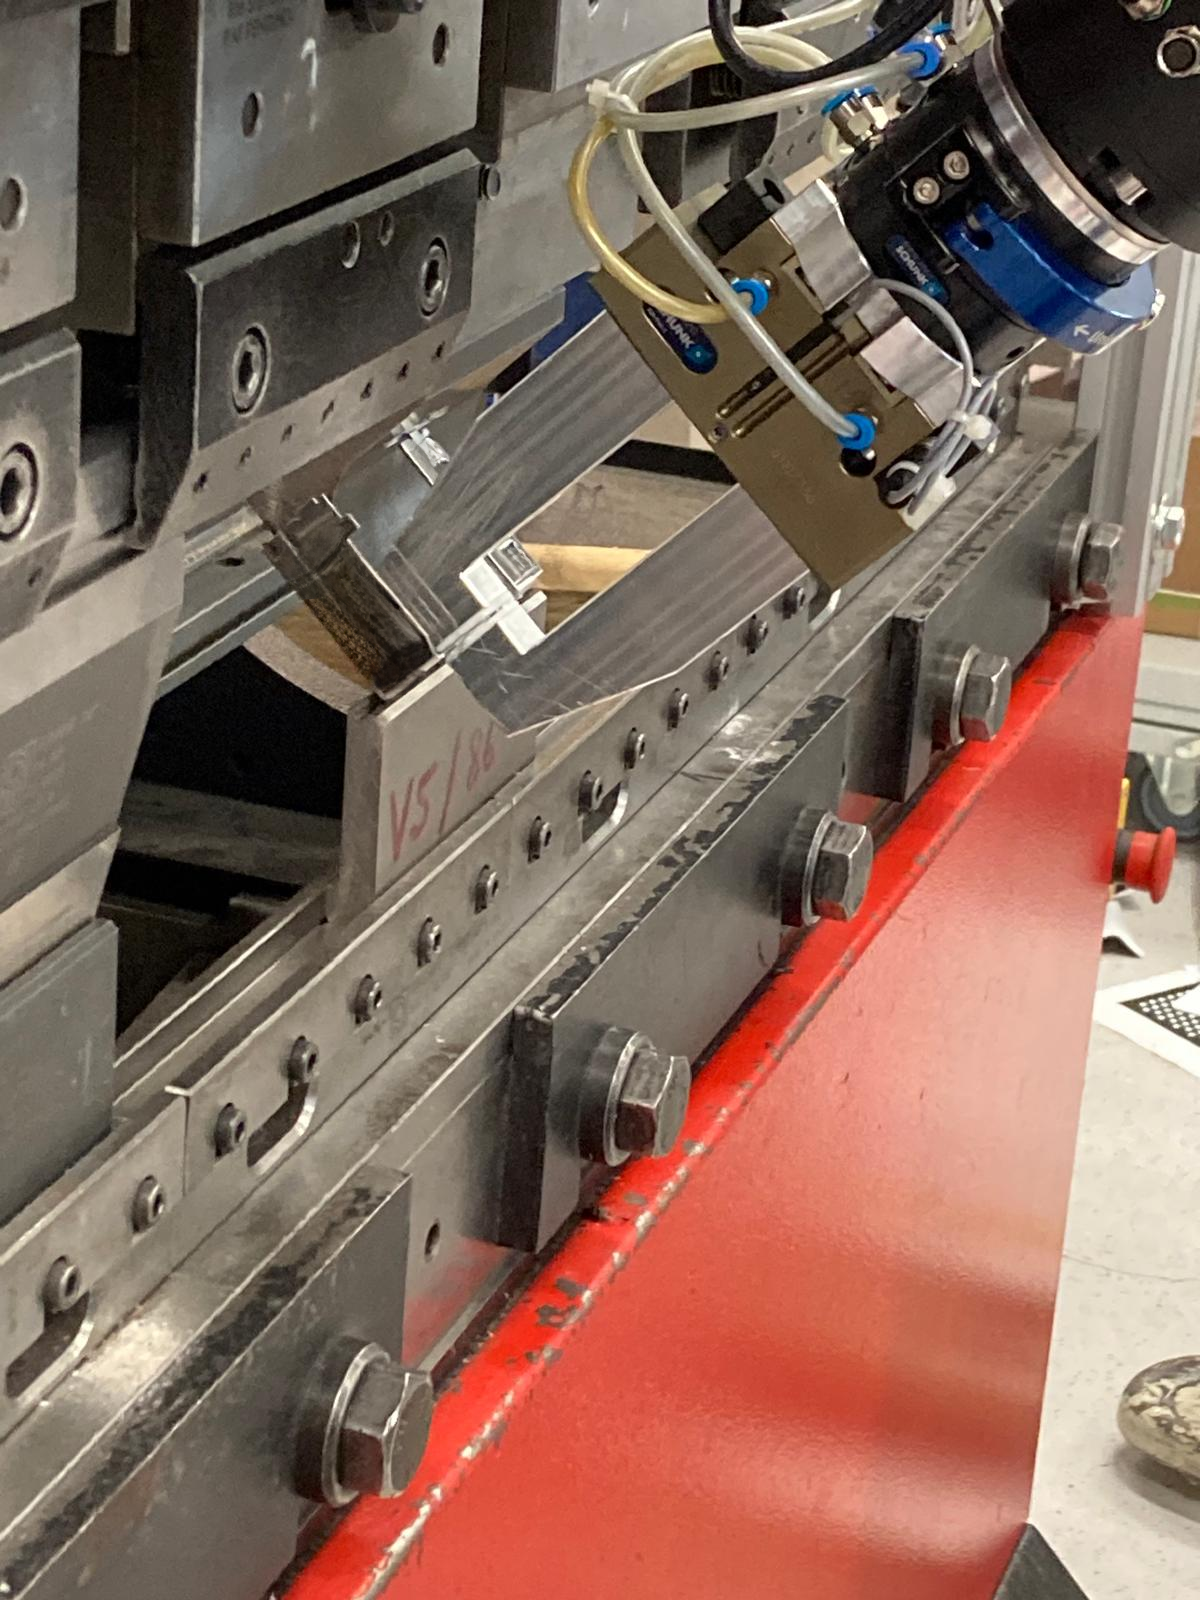
\includegraphics[width=\textwidth]{figures/bending/bending6-002.png}
        \caption{take away the bent sheet}
        \label{subfig:bending6-after}
    \end{subfigure}\hspace{0.1cm}
    \caption{Bending operation number 6 at bending station 1}
    \label{fig:bending-operation-6}
\end{figure}

Bending operation 5 and 6 are performed at bending station 1 as showing in figures \ref{fig:bending-operation-5} and \ref{fig:bending-operation-6} respectively. The process is similar to bending operation 1 as the robot doesn't hold the part during bending. Inspection is done after both bending operations. If after bending operation 6, the angle measurement is within tolerances, the current bending cycle is termed as successful.